\documentclass[12pt,a4paper,final,headinclude,footinclude,BCOR5mm]{scrartcl}

%%%%%%%%%%%%%%%%%%%%%%%%%%%%%%%%%%%%%%%%%
% Arsclassica Article
% Structure Specification File
%
% This file has been downloaded from:
% http://www.LaTeXTemplates.com
%
% Original author:
% Lorenzo Pantieri (http://www.lorenzopantieri.net) with extensive modifications by:
% Vel (vel@latextemplates.com)
%
% License:
% CC BY-NC-SA 3.0 (http://creativecommons.org/licenses/by-nc-sa/3.0/)
%
%%%%%%%%%%%%%%%%%%%%%%%%%%%%%%%%%%%%%%%%%

%----------------------------------------------------------------------------------------
%	REQUIRED PACKAGES
%----------------------------------------------------------------------------------------

\usepackage[
nochapters, % Turn off chapters since this is an article        
beramono, % Use the Bera Mono font for monospaced text (\texttt)
eulermath,% Use the Euler font for mathematics
pdfspacing, % Makes use of pdftex’ letter spacing capabilities via the microtype package
dottedtoc % Dotted lines leading to the page numbers in the table of contents
]{classicthesis} % The layout is based on the Classic Thesis style

\usepackage{arsclassica} % Modifies the Classic Thesis package
\usepackage[left=2cm,right=2cm,top=2cm,bottom=2cm]{geometry}

\usepackage[T1]{fontenc} % Use 8-bit encoding that has 256 glyphs

\usepackage[utf8]{inputenc} % Required for including letters with accents

\usepackage{graphicx} % Required for including images
\graphicspath{{Figures/}} % Set the default folder for images
\usepackage{wrapfig}

\usepackage{enumitem} % Required for manipulating the whitespace between and within lists

\usepackage{lipsum} % Used for inserting dummy 'Lorem ipsum' text into the template

\usepackage{subfig} % Required for creating figures with multiple parts (subfigures)

\usepackage{amsmath,amssymb,amsthm} % For including math equations, theorems, symbols, etc

\usepackage{varioref} % More descriptive referencing

%----------------------------------------------------------------------------------------
%	THEOREM STYLES
%---------------------------------------------------------------------------------------

\theoremstyle{definition} % Define theorem styles here based on the definition style (used for definitions and examples)
\newtheorem{definition}{Definition}

\theoremstyle{plain} % Define theorem styles here based on the plain style (used for theorems, lemmas, propositions)
\newtheorem{theorem}{Theorem}

\theoremstyle{remark} % Define theorem styles here based on the remark style (used for remarks and notes)

%----------------------------------------------------------------------------------------
%	HYPERLINKS
%---------------------------------------------------------------------------------------

\hypersetup{
%draft, % Uncomment to remove all links (useful for printing in black and white)
colorlinks=true, breaklinks=true, bookmarks=true,bookmarksnumbered,
urlcolor=webbrown, linkcolor=RoyalBlue, citecolor=webgreen, % Link colors
pdftitle={}, % PDF title
pdfauthor={\textcopyright}, % PDF Author
pdfsubject={}, % PDF Subject
pdfkeywords={}, % PDF Keywords
pdfcreator={pdfLaTeX}, % PDF Creator
pdfproducer={LaTeX with hyperref and ClassicThesis} % PDF producer
}

\hyphenation{Fortran hy-phen-ation}

%----------------------------------------------------------------------------------------
%	TITLE AND AUTHOR(S)
%----------------------------------------------------------------------------------------

\title{\normalfont\spacedallcaps{Amplificador Operacional NE5234}}

\author{\spacedlowsmallcaps{A. C. R. Tulic}}

\date{}

%----------------------------------------------------------------------------------------

\begin{document}

%----------------------------------------------------------------------------------------
%	HEADERS
%----------------------------------------------------------------------------------------

\renewcommand{\sectionmark}[1]{\markright{\spacedlowsmallcaps{#1}}} 
\lehead{\mbox{\llap{\small\thepage\kern1em\color{halfgray} \vline}\color{halfgray}\hspace{0.5em}\rightmark\hfil}} % The header style

\renewcommand*\contentsname{Contenido}
\renewcommand*\listfigurename{Figuras}
\renewcommand*\listtablename{Tablas}

\pagestyle{scrheadings} % Enable the headers specified in this block

%----------------------------------------------------------------------------------------
%	TABLE OF CONTENTS & LISTS OF FIGURES AND TABLES
%----------------------------------------------------------------------------------------

\maketitle % Print the title/author/date block

\setcounter{tocdepth}{2} % Set the depth of the table of contents to show sections and subsections only

\tableofcontents % Print the table of contents

\listoffigures % Print the list of figures

%----------------------------------------------------------------------------------------
%	DOCUMENTO
%----------------------------------------------------------------------------------------

\section{Análisis de la polarización}

\subsection{Fuentes de Corriente}

La figura \ref{634} presenta el diagrama esquemático del circuito de polarización del Op.Amp. NE5234.

\begin{figure}[!h]
\begin{center}
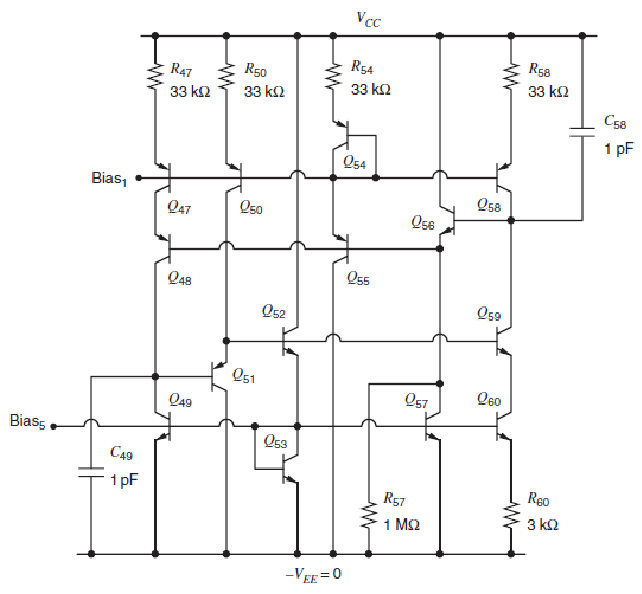
\includegraphics[width=400pt]{./imagenes/polne5234.png}
\end{center}
\caption{NE5234 bias circuit.}
\label{634}
\end{figure}

En la parte inferior de dicho circuito, los transistores $Q_{49}$ y $Q_{60}$ así como el resistor $R_{60}$ forman una fuente de corriente tipo WIDLAR. En dicha fuente, en lugar de conectarse al transistor $Q_{49}$ como diodo, las corrientes de base de $Q_{49}$ y $Q_{60}$ son proporcionadas por un separador (buffer) de ganancia unidad formado por los 4 transistores $Q_{50} \ldots Q_{53}$ intercalado desde el colector de $Q_{49}$. Este separador cumple la misma función que se le asigna a un transistor cuando reemplaza el corto circuito en las fuentes tipo espejo disminuyendo la corriente que se le extrae al colector de $Q_{49}$ (beta helper) y haciendo que $V_{CE49} = 2 V_{BEu}$ en lugar de $V_{BEu}$ como ocurre si $Q_{49}$ se conectara como diodo. Una de las razones por las que se utiliza este rebuscado circuito $Q_{50} \ldots Q_{53}$ es que si la técnica (beta helper) se llevara a cabo en forma tradicional con un único transistor, este aumento de $V_{CE49}$ generaría un necesario incremento en la tensión de alimentación $VCC$ de manera que los transistores que conducen la corriente de referencia de la fuente o corriente $I_{in}$ operasen en la región lineal fuera de saturación. A cambio de ello, para reducir el requerimiento de $VCC$ el aludido buffer  se conforma como un seguidor por emisor complementario lo cual significa que esta conformado por un par de transistores seguidores tipo pnp $Q_{50}$ y $Q_{51}$ y otro par de seguidores npn $Q_{52}$ y $Q_{53}$.  Si $V_{EB51} = V_{BE52}$ entonces en la ecuación de malla $V_{CE49} + V_{EB51} - V_{BE52} - V_{BE53} = 0$ el resultado es que $V_{CE49} = V_{BEu53}$ que reduce en aproximadamente $0,7 V$ el requerimiento de tensión de alimentación comparado con el circuito convencional. Similarmente los transistores seguidores complementarios $Q_{54} \ldots Q_{57}$ suministran las corrientes de base de los transistores $Q_{47}$ y $Q_{58}$ que conforman así otra fuente de corriente en este caso espejo. Asimismo, los transistores $Q_{48}$ y $Q_{59}$ operando en configuración base común y que conforman cascode con $Q_{47}$ y $Q_{60}$ reducen la dependencia de las corrientes en $Q_{47}$ y $Q_{60}$ respecto de la tensión de alimentación $VCC$.\\ 

\begin{wrapfigure}{r}{60mm}
\begin{center}
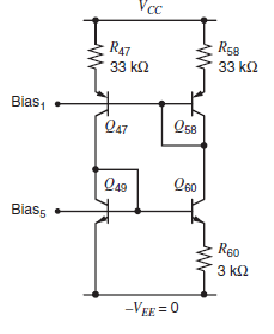
\includegraphics[width=150pt]{./imagenes/equiv.png}
\end{center}
\caption{Circuito equivalente de la figura \ref{634}}
\label{635}
\end{wrapfigure}

Para concentrarnos en la parte principal de este circuito de polarización se ha realizado su circuito equivalente en la figura \ref{635}, en donde se han removido las partes de \textit{beta helpers} y cascodes con sus elementos asociados.\\

Esta simplificación nos permite comprobar que el corazón de dicho circuito de polarización no es mas que una fuente de corriente autopolarizada utilizando a la tensión térmica que fuera ya estudiada en el apartado 5.6.9.3  del capitulo precedente en su figura 5.50.11.\\

En el circuito de la figura 5.50.11 se describe que los transistores $T_{3}$ y $T_{4}$ se encuentran apareados y también que el transistor $T_{2}$ posee dos emisores mientras que $T_{1}$ tiene solo uno, lo cual indica que el área de emisor de $T_{2}$ es el doble de la de $T_{1}$. Similares condiciones se mantienen en los circuitos de las figuras \ref{634} y \ref{635} en donde el área de emisor del transistor $Q_{60}$ es el doble de la correspondiente al $Q_{49}$. Como resultado de ello las corrientes de colector de dichos transistores pueden ser halladas, asumiendo $\beta$ y $V_{A}$ ambas infinito, aplicando la ecuación 33:

\begin{equation}
|I_{C47}| = I_{C49} = |I_{C58}| = I_{C60} = \dfrac{V_{T}}{R_{60}}ln(2) = \dfrac{0.026V}{3k\Omega}ln(2) = 6\mu A
\end{equation}

Si $R_{60}$ es constante estas corrientes resultan proporcionales a la temperatura absoluta (PTAT). Si bien en el circuito de las figuras \ref{634} y \ref{635} los betas y las tensiones de Early no son infinito, en la practica estas ecuaciones también proporcionan las correspondientes corrientes debido a la utilización de las técnicas de beta helpers y cascode oportunamente incorporadas. El circuito de polarización produce entonces dos tensiones de C.C. en los nodos rotulados $Bias1$ y $Bias5$, que son usados para establecer escalares copias de corriente de $6\mu A$ en los transistores pnp y npn del amplificador operacional, respectivamente. Así, mientras estas escalares copias de corriente de $6\mu A$ son proporcionales a la temperatura absoluta (PTAT), las transconductancias de los transistores que conducen estas corrientes resultan independientes de la temperatura.\\

El resistor $R_{57}$ en la figura \ref{634} esta previsto en el circuito de polarización para el caso que no se establezca corriente al aplicar la tensión de alimentación. Sin $R_{57}$ los transistores podrían permanecer cortados debido a que la diferencia de potencial entre el nodo $Bias1$  y masa se encuentra muy próximo a $VCC$. En cambio con la presencia de $R_{57}$ el transistor $Q_{55}$  lleva el potencial de $Bias1$ hacia abajo permitiendo el arranque de la conducción de corriente. En el estado estable, la corriente por $R_{57}$ causa un incremento de corriente en el transistor $Q_{56}$ produciendo un pequeño efecto de sobrecarga en la operación del circuito de polarización.\\

\subsection{Polarización de la etapa de entrada}

La figura \ref{636} presenta un esquema simplificado de la etapa de entrada del amplificador operacional. Dicho circuito muestra una estructura de cascode doblado en dos circuitos amplificadores diferenciales complementarios de modo de lograr una operación \textbf{rail to rail} en lo que respecta a la tensión de entrada de modo común en ambas polaridades y sin embargo la transconductancia de esta etapa de entrada resulta independiente de la tensión de entrada de modo común.\\

\begin{figure}[!h]
\begin{center}
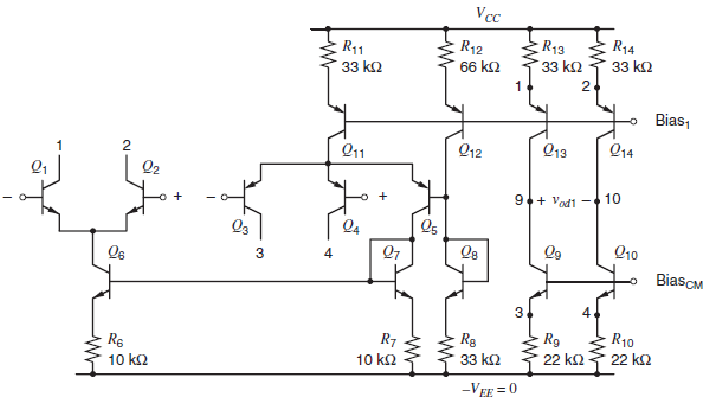
\includegraphics[width=400pt]{./imagenes/inputne5234.png}
\end{center}
\caption{Esquema simplificado de la etapa de entrada.}
\label{636}
\end{figure}

El nodo $Bias1$ perteneciente al circuito de polarización de la figura \ref{634}  y específicamente $Q_{58}$ y $R_{58}$ del mismo, en conjunto con el transistor $Q_{11}$ y resistor $R{11}$ de la figura \ref{636} forman una fuente de corriente espejo con resistencia de degeneración de emisor, de modo que en dicho circuito:

\begin{equation}
|I_{C11}| = \dfrac{R_{58}}{R_{11}}|I_{C58}| = \dfrac{33 k\Omega}{33 k\Omega}6\mu A = 6\mu A
\end{equation}

Similarmente, $|I_{C12}|=3\mu A$ y $|I_{C13}|=|I_{C14}|=6\mu A$ de modo que despreciando las corrientes de base por simplicidad, los $3\mu A$ provenientes de $Q_{12}$ circulan a través de $Q_{8}$ y $R_{8}$ fijando la tensión de la base de $Q_{5}$ con relación a masa en un valor de:

\begin{equation}
V_{B5} = |I_{C12}|R_{8} + V_{BE8} \approx 3 \mu A (33 k \Omega) - 7V = 0.8V
\end{equation}

Asumiendo que en la entrada del Op.Amp. se encuentre aplicada una tensión de entrada de modo común únicamente $V_{ic}$, los transistores $Q_{3}$ y $Q_{4}$ en conjunto pueden ser vistos formando una mitad del amplificador diferencial de entrada con $Q_{5}$ como la otra mitad del circuito. Este par diferencial se comporta como un amplificador totalmente desbalanceado por cuando $Q_{3}$ y $Q_{4}$ en conjunto tienen un área semiconductora de emisor (así como una corriente de saturación) mayor que la del transistor $Q_{5}$ causando una tensión de Off Set no nula. Despreciando esta tensión de Off Set por simplicidad, entonces si $V_{ic}$ es menor o igual a $0,8 V$, los $6 \mu A$ provenientes de $Q_{11}$ circulan en el par diferencial de entrada pnp $Q_{3}$ y $Q_{4}$ , y $Q_{5}$ y $Q_{7}$ así como el par diferencial de entrada npn $Q_{1}$ y $Q_{2}$  todos permanecen cortados. Por otro lado, si $V_{ic}$ es mayor o igual a $0,8 V$, el par diferencial de entrada pnp se encuentra cortado y los $6 \mu A$ de corriente provenientes de $Q_{11}$ circulan por $Q_{5}$ donde es copiada por la fuente de corriente espejo conformada por $Q_{7}$ y $Q_{6}$  para activar el par diferencial de entrada de npn $Q_{1}$ y $Q_{2}$.\\

En ambos casos extremos, la transconductancia de la etapa de entrada permanece constante, determinada por la corriente de polarización de $6 \mu A$. En la región de transición, alrededor de $V_{ic}$  igual a $0,8 V$, ambos pares diferenciales de entrada $Q_{1}$ y $Q_{2}$  así como $Q_{3}$ y $Q_{4}$  se encuentran activos. El ancho de dicha zona es de alrededor de $\pm 3 VT = \pm 78 mV$. En esta región, parte de los $6 \mu A$ provenientes de $Q_{11}$ circulan por el par  $Q_{3}$ y $Q_{4}$  y el resto circula por $Q_{5}$ quien finalmente polariza activamente el par $Q_{1}$ y $Q_{2}$ por intermedio de $Q_{6}$. Como consecuencia, la suma de las corrientes de $Q_{1}$ y $Q_{4}$ no es mas que los $6 \mu A$ ignorando a sus corrientes de base así como al efecto de modulación del ancho de la base y el desapareamiento. En tanto la transconductancia de cada par diferencial de entrada es proporcional a sus corrientes de polarización y dado que la transconductancia total de la etapa de entrada de este Op.Amp. es la suma de la correspondiente a ambos pares diferenciales, dicha transconductancia total no depende de la tensión de entrada de modo común $V_{ic}$.\\

Para obtener una alta ganancia de tensión en esta etapa de entrada, los transistores $Q_{9}$, $Q_{10}$, $Q_{13}$ y $Q_{14}$ de las fuentes de corriente que adicionan las salidas de ambos pares diferenciales complementarios, deben operar en su región activa, fuera de saturación a fin de presentar una alta resistencia de salida $roe$.\\

Así, mientras $Bias1$ es ajustado de modo que $|I_{C13}|=|I_{C14}|=6 \mu A$ BiasCM deberá ser ajustado de modo que $I_{C9}$ e $I_{C10}$ también sean exactamente de $6 \mu A$. Si acaso estas corrientes $I_{C9}$ e $I_{C10}$ fueran simplemente determinadas por este valor constante (y no hubiera modo de ajustar BiasCM) la tensión de modo común de salida en los nodos 9 y 10 se volvería muy sensible a pequeños desapareamientos entre los transistores $Q_{9},Q_{10},Q_{13}$ y $Q_{14}$. Por ejemplo, suponiendo que por $Q_{9}$ y $Q_{10}$ circularan los $6 \mu A$ como se esperaba pero por $Q_{13}$ y $Q_{14}$ la corriente fuese de unos $6.1 \mu A$ cada uno causado por un pequeño incremento en el área semiconductora de sus emisores, entonces la tensión de salida de modo común se incrementaría con el objeto de que se satisfaga la ley de Kirchoff en los nodos 9 y 10 forzando a los transistores $Q_{13}$ y $Q_{14}$ a operar en su región de saturación para hacer bajar sus corrientes a $6 \mu A$. Similarmente si $Q_{9}$ y $Q_{10}$ impulsaran corrientes levemente superiores a las correspondientes a $Q_{13}$ y $Q_{14}$ la tensión de salida de modo común debería caer hasta que se alcance a cumplir la ley de Kirchoff en los nodos referidos. La situación asi descripta determina que la tensión de salida de modo común no se encontraría bien controlada en el circuito de la figura \ref{636} correspondiente a esta primera etapa. Este problema es superado por intermedio de la segunda etapa del Op.Amp. la cual ajusta el valor de BiasCM de modo de determinar la tensión de salida de modo común en el valor adecuado para que los transistores $Q_{9},Q_{10},Q_{13}$ y $Q_{14}$ todos operen fuera de saturación.

\subsection{Polarización de la segunda etapa del Op.Amp.}

La figura \ref{637} presenta el circuito esquemático de la segunda etapa del NE5234. Los nodos 9 y 10 son los terminales de salida de la primera etapa y por consecuencia la entrada de esta segunda. Los capacitores $C_{21}$ y $C_{22}$ son utilizados para introducir compensación de frecuencia y evitar así perjudiciales oscilaciones, tema que se tratara oportunamente. El otro terminal del capacitor $C_{22}$ se conecta en la salida del Op.Amp. como se vera al estudiar su etapa de salida. Ambos capacitores son ignorados en el presente análisis. Las configuraciones seguidor por emisor de los transistores $Q_{21}$ y $Q_{22}$ tienen por objeto reducir la carga de la segunda etapa sobre la primera. Para un primer análisis ignore la presencia de $Q_{23}$ y $Q_{24}$ ya que los mismos se encuentran normalmente cortados (protecciones). Los transistores $Q_{25},Q_{26},Q_{27}$ y $Q_{28}$ forman un par diferencial en el cual cada rama del par diferencial se compone de dos transistores. Este par diferencial tiene por objetivo amplificar la tensión de salida diferencial de la primera etapa $v_{od1}$ y su desdoblamiento permite obtener dos salidas, ambas en fase entre si, una sobre el nodo 25 y la otra en el nodo 26, tal como es requerido por la etapa de salida.\\

\begin{figure}[!h]
\begin{center}
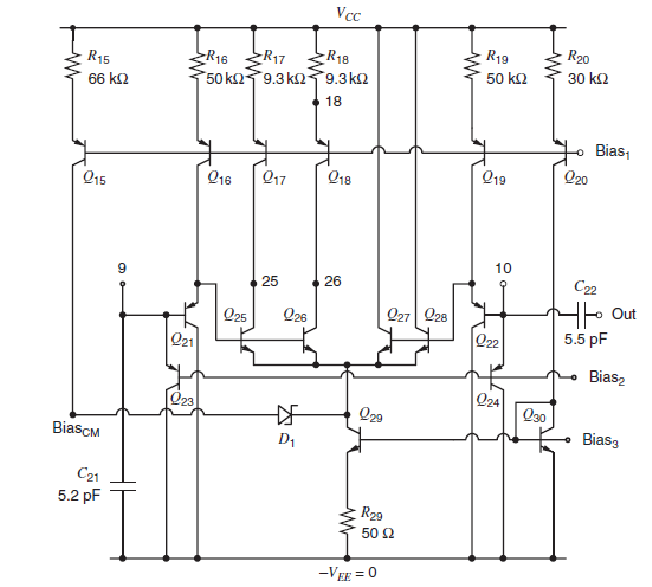
\includegraphics[width=400pt]{./imagenes/secondne5234.png}
\end{center}
\caption{Esquema de la segunda etapa del NE5234.}
\label{637}
\end{figure}

De la misma forma como se describiera en la primera etapa, ahora $Q_{15}$ y $R_{15}$ en conjunto con $Q_{58}$ y $R_{58}$  del circuito de polarización de la figura 6.34, forman una nueva fuente de corriente no simétrica de modo de establecer una corriente de

$$|I_{C15}| = \dfrac{R_{58}}{R_{15}}|I_{C58}| = \dfrac{33 \Omega}{66 k\Omega}6 \mu A = 3 \mu A$$

Similarmente

$$|I_{C16}| = |I_{C19}| = 4 \mu A$$
$$|I_{C17}| = |I_{C18}| = 21 \mu A$$

y también

$$|I_{C20}| = 6.6 \mu A$$

Por simplicidad asuma que $I_{C19}$ e $I_{C16}$ determinan que $V_{EB21} = V_{EB22} = 0,7 V$. Despreciando las corrientes de base, la corriente $I_{C15}$ circula a través del diodo Schotky $D1$ determinando que la diferencia de potencial que aparece entre bornes de dicho diodo sea

$$V_{D1} = V_{T} ln \left \{ \frac{|I_{C15}|}{Is(D1)} \right \}$$

en donde $IS(D1)$ es la corriente de saturación inversa de dicho diodo. Tomando a dicha corriente en un valor de $6*10^{-13} A$, dicha tensión resulta

$$V_{D1} = 0.026 \left \{ \frac{3*10^{-6}}{6*10^{-13}} \right \} = 0.4 V$$

El resistor $R_{29}$ en conjunto con los transistores $Q_{29}$ y $Q_{30}$ conforman una fuente de corriente WIDLAR y como sabemos la ecuación de malla en la que intervienen los diodos base emisor de esta fuente

$$V_{T} ln \left \{ \frac{I_{C30C}}{I_{S30}} \right \}             ln(/)-V_{T} ln(I_{C29C}/I_{S29})-I_{C29}R_{29} = 0$$

En el Op.Amp. NE5234 la relación $IS29/IS30 = 7$ por lo que

$$V_{T} ln(7 I_{C30C}/I_{c29}) = I_{C29}R_{29}$$

Dado que $I_{C30} = I_{C20} = 6,6 \mu A$ la solución por prueba y error de esta ecuación arroja como resultado una corriente $I_{C29} =  42 \mu A$. En consecuencia la corriente disponible para activar a los transistores $Q_{25}$, $Q_{26}$, $Q_{27}$ y $Q_{28}$ es  $I_{C29} - I_{D1} =  39 \mu A$. Digamos que $V_{9}$ y $V_{10}$ representen los potenciales de los nodos 9 y 10 contra masa y aceptemos que $V_{9} = V_{10}$. Entonces

$$I_{C25} = I_{C26} = I_{C27} = I_{C28} = \dfrac{39}{4} \mu A \approx 10 \mu A$$

Por simplicidad asuma que estas corrientes determinan también que

$$V_{BE25} = V_{BE26} = V_{BE27} = V_{BE28} = 0.7 V$$

Digamos ahora que $V_{cmout1}$ represente la tensión de modo común de salida de la primera etapa incluyendo tanto su componente de continua como la componente de señal. Esta tensión es el valor medio de las tensiones presentes en los nodos 9 y 10, es decir

$$V_{cmout1} = \frac{1}{2} (V_{9} + V_{10})$$

Similarmente digamos que Vbiascm represente la tensión del nodo BiasCM  con referencia a la masa. Principios de funcionamiento de la primera y segunda etapa determinan conjuntamente a ambas tensones, como se anticipó precedentemente y se pasa a describir detalladamente a continuación.\\

Considere la primera etapa en donde $V_{biascm}$  y $V_{cmout1}$ son respectivamente una tensión de entrada y la otra de salida de la misma. La relación entre estas dos tensiones esta determinada por la transferencia del amplificador emisor común con resistencia de degeneración en su emisor ($Q_{9}$ y $Q_{10}$) y su carga activa ($Q_{13}$ y $Q_{14}$). Digamos que  $V_{biascm}, V_{9}, V_{10}$  representen  a los cambios en las tensiones entre los nodos BiasCM, 9 y 10  con referencia a masa, respectivamente. Llamemos asimismo A a la ganancia de pequeña señal definida por el cociente (v9/vbiascm ), entonces también  $A = vbiascm/v10$ debido a la simetría. En otras palabras A es la ganancia de tensión de modo común establecida entre el nodo BiasCM y la salida de la primera etapa. La polaridad de esta ganancia A es negativa ya que si se incrementa la tensión del nodo BiasCM esto aumenta las corrientes de $Q_{9}$ y $Q_{10}$ reduciendo la tensión de salida de modo común. La magnitud de la ganancia A es grande pero no será calculada en esta oportunidad por cuanto su valor no es importante para realizar un estudio de primera aproximación para hallar los puntos de operación. Asuma que A es infinito cuando $Q_{9},Q_{10},Q_{13}$ y $Q_{14}$ operan en su zona activa y lineal.\\

Asuma que la tensión de entrada de modo común del amplificador operacional $V_{ic}$ es mucho menor que los $0,8 V$ de umbral antes definido. Entonces $Q_{1}$ y $Q_{2}$ se encuentran cortados. Mientras las diferencias de potencial de C.C. sobre las resistencia $R_{13}$ y $R{14}$ son

$$|I_{C13}|=|I_{C14}|=6 \mu A$$
$$V_{R13} = V_{R14} = 6 \mu A (33 k \Omega) = 0.2 V$$

Si, $V_{CE13(sat)} = V_{CE14(sat)} = -0.1 V$, $Q_{13}$ y $Q_{14}$ operan en la región lineal mientras $V_{cmout1}$ este por debajo de $VCC – 0,3 V$.\\

Para cumplimentar la ley de Kirchoff en los nodos 9 y 10, $Q_{9}$ y $Q_{10}$ deben adaptarse y conducir la misma corriente impuesta por los transistores $Q_{13}$ y $Q_{14}$ la cual es de $6 \mu A$ bajo condiciones nominales. Asumamos que estas corrientes determinan que las tensiones $V_{BE9} = V_{BE10} = 0,7 V$. También, mientras vic sea menor o igual a $0,8 V$ y la corriente de C.C. a través de $R_{9}$ y $R_{10}$  es

$$I_{R9} = I_{R10} = I_{C9}$$
$$I_{C3} = I_{C10}$$
$$I_{C4} = 9 \mu A$$

y como resultado la tensión de C.C. sobre estas resistencias es

$$V_{R9} = V_{R10} = 9 \mu A (22 k \Omega) = 0.2 V$$

Asumamos que $V_{CE9(sat)} = V_{CE10(sat)} = 0.1 V$. Entonces $Q_{9}$ y $Q_{10}$ operan en la región activa y si $V_{cmout1}$ es mayor a $0,3 V$ entonces $V_{biascm}$ es

$$V_{biascm} = V_{R9} + V_{BE9} = V_{R10} + V_{BE10} = 0.9 V$$

Este comportamiento esta resumido en la grafica de la figura \ref{638} en donde se presentan dos curvas de $V_{cmout1}$ en relación a $V_{biascm}$ una de ellas rotulada como Características del Amplificador. Para $V_{biascm}$ menor que $0,9 V$ ella describe que $V_{cmout1}$ permanece constante en un valor $VCC – 0,3 V$ por cuanto $Q_{13}$ y $Q_{14}$ saturan.  Para $V_{biascm} > 0,9 V$  esta curva describe que  Vcmout1  permanece constante en un valor $0,3 V$ por que $Q_{9}$ y $Q_{10}$ saturan. Para $V_{biascm}$ igual a $0,9 V$ $V_{cmout1}$ cae desde  $VCC – 0,3 V$ a  $0,3 V$  por cuanto $A = - \infty$ como se asumió previamente.\\

\begin{figure}[!h]
\begin{center}
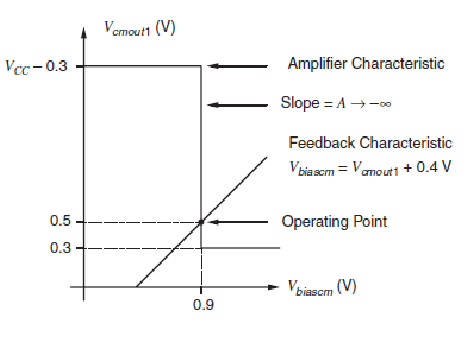
\includegraphics[width=250pt]{./imagenes/curvasvcmout1.png}
\end{center}
\caption{Curvas de $V_{cmout1}$ en relación a $V_{biascm}$.}
\label{638}
\end{figure}

La \ref{638} representa las curvas de $V_{cmout1}$ en relación a $V_{biascm}$. La característica del Amplificador originada en la primer etapa y la características de realimentación  derivada de la segunda etapa.\\

Ahora considere la segunda etapa, en esta la $V_{cmout1}$ es la tensión de entrada, mientras que $V_{biascm}$ es la de salida. Asumamos que en la primer etapa la tensión de salida de modo común se incrementa en vcmout1 . Entonces la tensión  entre los emisores de los transistores $Q_{21}$ y $_{Q22}$ y masa también se incrementa en aproximadamente vcmout1 por cuanto estos transistores se comportan como seguidores por emisor. Estos cambios causan que la tensión entre el colector del transistor $Q_{29}$ y masa se eleve también aproximadamente vcmout1 por cuanto las tensiones entre base y emisor de los transistores $Q_{25}$ - $Q_{28}$ permanecen casi constantes. Estos resultados se originan en el hecho de que  la combinación de $Q_{21}$ y $_{Q26}$ por un lado y $Q_{27}$ y $_{Q28}$ por otro forman un par diferencial. Mientras la entrada de este par diferencial es una señal de modo común pura bajo las condiciones descriptas precedentemente, las corrientes de colector de cada uno de estos transistores individualmente son aproximadamente constantes asumiendo que la fuente de corriente de polarización $Q_{29}$ posee una alta resistencia de salida. Además, desde el punto de vista de las componentes de C.C, los seguidores de emisor $Q_{21}$ y $_{Q22}$ modifican los niveles de tensión  $V_{9}$ y $V_{10}$ hacia arriba en $0,7 V$. y el par diferencial desdoblado $Q_{25}$ - $_{Q28}$ cambia el nivel de la salida del seguidor por emisor hacia abajo en la misma cantidad. En consecuencia por cuanto la caída de tensión sobre el diodo Schotky permanece constante, la tensión entre el nodo BiasCM y masa es la tensión de modo común de salida de la primera etapa modificada hacia arriba en $0,4 V$. Mientras que la tensión de colector de $Q_{29}$ se eleva en $V_{cmout1}$ en este ejemplo, la tensión entre el nodo $BiasCM$ y masa se eleva en la misma cantidad. Como resultado la tensión entre el nodo $BiasCM$ y masa es

$$V_{biascm} = V_{cmout1} + 0.4V$$

Esta ecuación se ha representado gráficamente en la figura \ref{638}. En dicha figura su representación se ha rotulado como Característica de Realimentación (Feedback Characteristic) por cuanto la función de la segunda etapa es tomar una muestra o censar, modificar el nivel y retornar hacia la primera etapa la tensión de salida de modo común para controlar el punto de operación del modo común. Dicho lazo es un ejemplo de realimentación negativa por cuanto si se produjese un aumento de $V_{cmout1}$ ello aumenta vbiascm lo cual entonces reduce $V_{cmout1}$ mediante la operación del amplificador de modo común de ganancia A mencionado al describir el circuito de la primera etapa. No obstante lo dicho cabe aclarar que este lazo de realimentación negativa actúa sobre la tensión de modo común de salida de la primera etapa y no tiene ninguna influencia sobre la tensión de salida de modo diferencial de dicha primera etapa. Por ejemplo, suponga que la tensión $V_{9}$ se modifica incrementalmente y la tensión $V_{10}$ cambia disminuyendo la misma cantidad. Entonces la tensión entre el nodo 29 y masa permanece constante ya que $Q_{25}$ y $_{Q26}$ tendería a aumentarla mientras que $Q_{27}$ y $_{Q28}$ haría lo propio pero para disminuirla y con igual intensidad. Como resultado de ello vbiascm permanece constante y el lazo inactivo. Es por ello que el citado lazo es denominado Lazo de Realimentación de Modo Común.\\

La figura \ref{638} presenta un análisis gráfico para describir como se alcanza el punto de polarización. Dos variables son las principales en este análisis $V_{cmout1}$ y $V_{biascm}$. Cada una de estas variables influye sobre la otra de dos formas o caminos: por las características del Amplificador y del Lazo de Realimentación antes descritos. Cuando ambas características se satisfacen el dispositivo opera en el punto de intersección de dichas curvas características donde el valor medio de $V_{biascm} = 0,9 V$ y el valor medio de $V_{cmout1} = 0,5 V$. En principio, un A finito, $V_{EB21} = V_{EB22}$  diferentes a $V_{BE25} = V_{BE26} = V_{BE27} = V_{BE28}$ altera el punto de operación ligeramente, pero $Q_{9},Q_{10},Q_{13}$ y $Q_{14}$  en la practica todavía operan en su región activa para un amplio rango de condiciones del proceso, fuentes de alimentación y rangos de temperatura.

\subsection{Análisis de C.C. de la etapa de salida}

En muchos amplificadores operacionales la etapa de salida es una configuración colector común, tal como se viera en el 741. En este ultimo dicha configuración permite obtener el bajo valor deseado de resistencia de salida y una muy buena eficiencia en el manejo de energía pero la principal limitación de dicha configuración es su baja capacidad de excursión ya que su tensión de salida puede variar entre 1,4 V por arriba de la tensión de alimentación negativa (–VEE + 1,4) hasta 0,8 V por debajo de la tensión de alimentación positiva (VCC – 0,8). Estas características no constituyen serias limitaciones cuando las tensiones de alimentación pueden llegar hasta unos +/- 15 o 20 V, pero significaría excursión prácticamente nula si la alimentación fuera de VCC = +2 V y VEE = 0 V.\\

Para superar estas limitaciones el amplificador operacional NE5234 no utiliza transistores en configuración colector común para excitar a su terminal de salida. En la figura \ref{639} se presenta el diagrama esquemático de su etapa de salida. Los nodos 25 y 26 son los terminales de entrada de esta etapa y coinciden con los de salida de su segunda etapa. Allí los capacitores $C_{25}$ y $C_{26}$ en serie con los resistores $R_{25}$ y $R_{26}$ son los circuitos de compensación de frecuencia que evitan oscilaciones y no serán tenidos en cuenta en este estudio.

\begin{figure}[!h]
\begin{center}
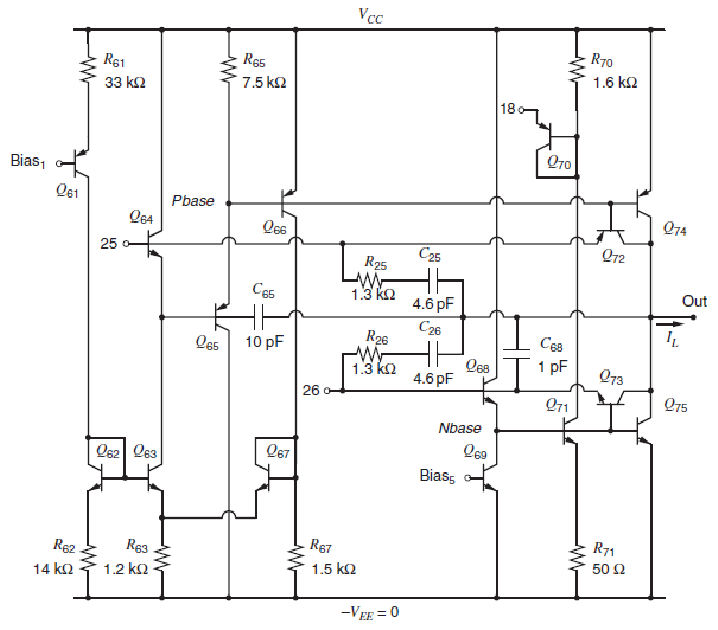
\includegraphics[width=400pt]{./imagenes/salida5234.png}
\end{center}
\caption{Etapa de salida del NE5234.}
\label{639}
\end{figure}

La salida es excitada por los transistores $Q_{74}$ y $Q_{75}$ que operan en configuración emisor común. Resultado de dicha configuración, la resistencia de salida de esta etapa es alta pero la misma se baja dramáticamente mediante aplicación de realimentación negativa por fuera del Op.Amp. La principal razón para utilizar este tipo de etapa de salida es que ello puede excitar a su terminal de salida en un rango de tensión que va desde $V_{CE75(sat)}$ o cerca de $0,1 V$ por arriba de la tensión de alimentación baja hasta $V_{CE74(sat)}$ o nuevamente $0,1 V$ por debajo de la tensión de alimentación mas alta. En otras palabras esta etapa permite obtener una excursión de salida del tipo rail to rail.\\

El objetivo de diseño es lograr que el transistor $Q_{74}$ este en condiciones de enviar $10 \mu A$ hacia el terminal de salida. Similarmente, $Q_{75}$ debería estar en condiciones de enviar los mismos $10 \mu A$ hacia la carga. La corriente de polarización de los transistores $Q_{25}$ y $Q_{26}$ en la figura \ref{637} es de alrededor de $10 \mu A$ cada una. Para este limite requerido de circulación de corriente hacia o desde los terminales 25 y 26 de dicho circuito, la ganancia de corriente de la etapa de salida debe ser de aproximadamente 1000. Para alcanzar este requerimiento cuando el transistor $Q_{75}$ impulsa corriente hacia la carga se emplea el seguidor de emisor $Q_{68}$. La ganancia de corriente entre el terminal 26 y el de salida es aproximadamente $\beta_{75}*\beta_{68} = \beta^{2}(npn)$ que alcanza un valor mas grande que 1000 por cuanto el mínimo valor de la ganancia de corriente de un transistor npn $\beta^{2}(npn)$ es de 40 para este proceso de fabricación. Por otro lado cuando el transistor $Q_{74}$ impulsa corriente hacia la carga, la ganancia de corriente podría ser menor que 1000 si $Q_{74}$ fuera únicamente excitado con un seguidor por emisor ya que la ganancia de corriente de los transistores pnp puede llegar a tener un valor mínimo de 10 en dicho proceso. Para superar este inconveniente el separador que excita la base del transistor $Q_{74}$ es un seguidor por emisor complementario $Q_{64}$ - $Q_{65}$ consiguiendo una ganancia de corriente entre el terminal 25 y el de salida que resulta aproximadamente $\beta_{64}*\beta_{65}*\beta_{74} = \beta^{2}(npn)$.\\

Los nodos rotulados $Bias1$ y $Bias5$ son los mismos que se han observados en la figura \ref{634}. Desde el punto de vista de C.C. dada la fuente espejo también puede aplicarse

$$|I_{C61}| = \frac{R_{58}}{R_{61}}|I_{C58}| = \frac{33 k\Omega}{33 k\Omega} * 6 \mu A = 6 \mu A$$


Los transistores $Q_{62}$ y $Q_{63}$ en conjunto con los resistores $R_{62}$ y $R_{63}$ forman una nueva fuente de corriente espejo no simétrica y en ella se observa que 

$$|I_{C63}| = \frac{R_{62}}{R_{63}} * 6 \mu A = 70 \mu A$$

Sin embargo dicha relación se basa en que la diferencia de potencial en $R_{62}$ y en $R_{63}$ son idénticas, ya que la diferencia de potencial en los diodos base emisor de $Q_{62}$ y $Q_{63}$ es despreciable. Con las corrientes calculadas precedentemente, la diferencia entre las tensiones base-emisor de los transistores , asumiendo que los mismos son idénticos, resultan ser:

$$V_{T} * ln(I_{C62}/I_{C63}) = 64 mv$$

mientras la diferencia de potencial sobre $R_{62}$ resulta ser $(6 \mu A * 14 k\Omega) = 84 mV$, aquí las diferencias entre las tensiones base emisor antes calculada no resulta despreciable por lo que corresponde plantear la ecuación de la ley de Kirchoff considerando betas infinitos, o sea

\begin{equation}
I_{C62}*R_{62} - I_{C63}*R_{63} = V_{BE63} - V_{BE62} = V_{T} *  ln(I_{C63}/ I_{C62})
\label{z}
\end{equation}


Así resolviendo por prueba y error el resultado es que  $I_{C63} = 33 \mu A$ y despreciando las corrientes de base también  $I_{C64} = I_{C63} = 33 \mu A$. La corriente en $R_{65}$ es $I_{R65} = V_{EB74} / R_{65}$  y resulta igual a $I_{C65}$ despreciando las corrientes de base. En la practica, $V_{EB74}$ depende de $I_{C74}$. Un caso en que $I_{C74}$ es grande ( mayor que $1 \mu A$) es considerado mas adelante. En dicho caso, $V_{EB74}$ es también grande. Por ejemplo $V_{EB74} = 0,75 V$. Por lo tanto 

$$|I_{C65}| = I_{R65} = 100 \mu A$$

Mientras las tensión base-emisor del transistor $Q_{69}$ es igual a aquella de $Q_{49}$ en la figura \ref{634}, las corrientes $I_{C69} = I_{C49} = 6 \mu A$. Despreciando las corrientes de base, también $I_{C68} = I_{C69} = 6 \mu A$. Sin embargo considerando dichas corrientes de base no nulas, las mismas tienen a menudo una influencia significativa en el comportamiento de la etapa de salida, especialmente sobre $I_{C64},I_{C65}$ e $I_{C68}$, las cuales serán recalculadas tiempo después de haber determinado $I_{C74}$ e $I_{C75}$. Los transistores $Q_{70}, Q_{72}$ y $Q_{73}$ normalmente operan cortados y en principio no serán considerados. 

\begin{figure}[!h]
\begin{center}
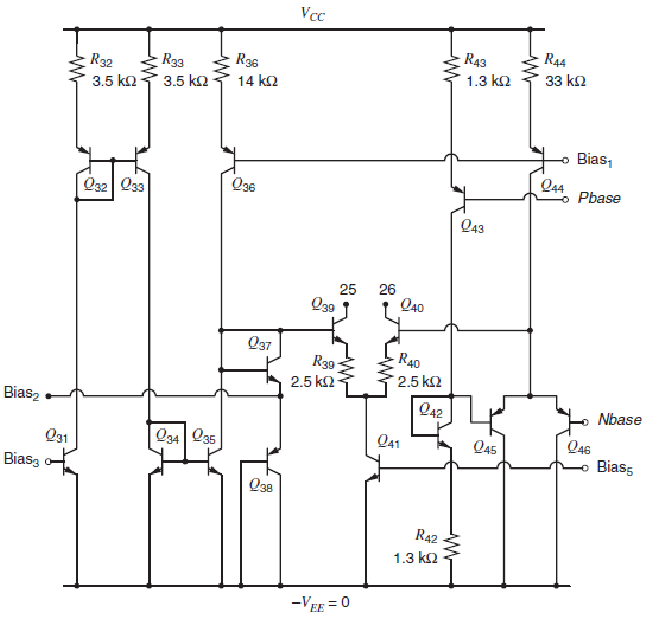
\includegraphics[width=300pt]{./imagenes/biasoutput.png}
\end{center}
\caption{Etapa de salida (bias circuit).}
\label{640}
\end{figure}

Las corrientes de C.C. de los otros transistores integrantes de la etapa de salida están determinadas por el circuito de polarización de dicha etapa que se representa en la figura \ref{640}. Los nodos $Pbase$ y $Nbase$ son los terminales de salida de la etapa de salida y constituyen las entradas a dicho circuito de polarización. El nodo $Bias2$ es una salida que se transforma en entrada en el circuito de la segunda etapa de la figura \ref{637} y no será considerado en un principio. El nodo $Bias3$ proviene de la segunda etapa. $V_{BE31} = V_{BE30}$, $I_{C31} = I_{C30} = 6,6 \mu A$. Esta corriente es copiada por las configuraciones espejo $Q_{32}$ - $Q_{33}$  y $Q_{34}$ - $Q_{35}$ de modo que $I_{C35} = 6,6 \mu A$ despreciando las corrientes de base y la modulación del ancho de la base. Aplicando la relación de Widlar arroja  $I_{C44} = 6 \mu A$. Similarmente $I_{C36}  = (R58/R36) * 6 \mu A = 14 \mu A$.\\

Entonces $I_{C37} = I_{C38} = I_{C36} = I_{C35} = 7,4 \mu A$. El nodo $Bias5$ proviene del circuito de polarización de la figura \ref{634}. En consecuencia $V_{BE41} = V_{BE49}$ y como en el NE5234 $(I_{S41} / I_{S49}) =  3$, $I_{C41} = 3*I_{C49} = 18 \mu A$.\\

Para describir la interacción entre los circuitos de las figuras \ref{639} y \ref{640}, la figura \ref{641} presenta un diagrama esquemático simplificado de la etapa de salida del NE5234 incluyendo su circuito de polarización. Por simplicidad en dicho circuito todos los transistores que normalmente se encuentran cortados no se han incluido y las corrientes de polarización que se han calculado precedentemente se encuentran representadas mediante generadores independientes de corriente. Como en muchas etapas de salida también en este caso la etapa de salida opera en \textbf{clase AB}. Sin embargo las relaciones básicas entre las corrientes de colector del par de transistores de salida es diferente aquí, comparado con aquellas correspondientes a la mayoría de las etapas de salida de muchos Op.Amp., tal como se detallará mas adelante.\\

En amplificadores operacionales cuyas etapas de salida se encuentran constituidas por transistores operando en clase AB Clásica, la técnica de polarización consiste en imponer que el producto de las corrientes de polarización de los dos transistores de salida como una constante. Tal el caso del Op. Amp. 741 en donde el par de salida $Q_{14}$ y $Q_{20}$ se encuentran polarizados mediante el circuito conformado por los transistores $Q_{18}$ y $Q_{19}$ y como se recordara, el planteo de la ley de Kirchoff sobre la malla donde intervienen las tensiones base-emisor de todos dichos transistores arrojaba la ecuación:

\begin{figure}[!h]
\begin{center}
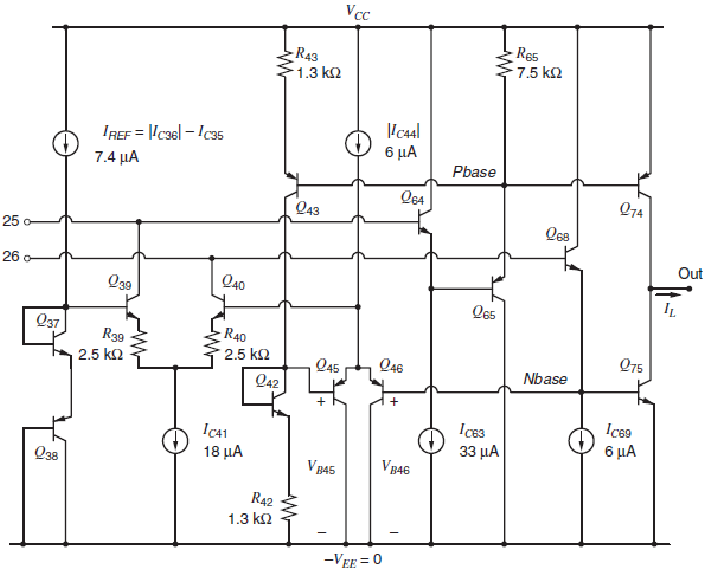
\includegraphics[width=300pt]{./imagenes/neoutputbias.png}
\end{center}
\caption{Etapa de salida del NE5234 con bias circuit.}
\label{641}
\end{figure}

lo cual implica que ninguna de las dos corrientes ni $I_{C14}$ ni $I_{C20}$ pueden anularse cuando la restante se hace grande. Sin embargo en la ecuación de Kirchoff en la mencionada malla se han despreciado algunos términos por simplicidad. Por ejemplo las caídas de tensión que aparecen en las resistencias no nulas de las regiones de base y de emisor del par de transistores de salida. Estas caídas extra incrementan la magnitud de la tensión $V_{BE}$ del transistor excitador, en forma proporcional al aumento de la corriente por la carga enviando al corte al transistor inactivo en algún punto. Como resultado de ello se produce un incremento en el tiempo requerido para volver hacia atrás la operación de dicho transistor y se empeora la distorsión de cruce.\\

Para superar este inconveniente los transistores de la etapa de salida del amplificador operacional NE5234 se encuentran polarizados de modo que nunca pueden cortarse aun en los extremos de excursión máxima de la tensión de salida. El circuito compara las corrientes de los dos transistores de salida y controla la pequeña corriente a través del lazo de realimentación negativa cuando la corriente de salida es grande. Dicha corriente de salida puede ser sensada incorporando elementos en serie con el colector o el emisor del transistor de salida. Sin embargo la caída de tensión a través de dichos elementos podría no ser nula y reduciría la excursión de la tensión de salida. Entonces para optimizar dicha excursión de salida estas corrientes son sensadas por intermedio de las tensiones base-emisor de los transistores de salida. Estas tensiones son manipuladas y enviadas al par diferencial $Q_{45}-Q_{46}$ para su comparación. Este amplificador diferencial opera sobre las tensiones de las bases de dichos transistores $V_{B45}$ y $V_{B46}$. Para $V_{B46}$:

$$V_{B46} = V_{BE75} = V_{T} ln(I_{C75}/I_{S75})$$

En otras palabras, la función logaritmo natural mapea la corriente de colector de $Q_{75}$ en comparación con su tensión base-emisor la cual es igual a la tensión $V_{B46}$ por la ecuación de malla de Kirchoff.

Por medio de $V_{B45}$, las variaciones de la tensión emisor-base de $Q_{74}$ es convertida en variaciones de corriente de colector del transistor $Q_{43}$ y vuelta atrás a través de $Q_{42}$ y $R_{42}$. Entonces de acuerdo a Kirchoff:

$$v_{B45} = V_{BE42} + I_{C43}*R_{42}$$

donde:

$$I_{C43} = \frac{V_{EB74}-V_{EB43}}{R_{43}}$$

como $R_{42} = R_{43}$ sustituyendo la ultima en la anterior se obtiene:

\begin{equation}
V_{B45} = V_{BE42} + V_{EB74} - V_{EB43} = V_{EB74} + V_{T} * ln \frac{I_{S43}}{I_{S42}} = V_{T} * ln \frac{I_{C74}}{I_{S75}}
\label{a}
\end{equation}

en donde se ha asumido que

$$I_{S75} = \frac{I_{S74}*I_{S42}}{I_{S43}}$$

Dicha ecuación expresa que $V_{B45}$ es igual a la tensión base-emisor del transistor equivalente $Q_{75}$ cuya corriente de colector es $I_{C74}$. Esta conversión permite que   $I_{C74}$ sea comparada con $I_{C75}$ por $Q_{45} – Q_{46}$ en un modo no sensible a las diferencias entre las corrientes de saturación de los transistores pnp y npn. Si:

$$|V_{B45} - V_{B46}| > 3 V_{T}$$

en el par de transistores, el que mayor tensión de base alcance pasara a funcionar al corte. Bajo esta condición, la tensión de los emisores de estos transistores contra tierra es controlada por aquel transistor de salida que conduzca la mayor corriente. Esta tensión redirige la entrada sobre una de las ramas del amplificador diferencial $Q_{39} – Q_{40}$. La otra entrada presenta una tensión constante dispuesta por $I_{REF} = I_{C36} - I_{C35}$  circulando por los transistores conectados como diodo $Q_{37}$ y $Q_{38}$. Los transistores $Q_{39}$ y $Q_{40}$ forman el corazón del amplificador diferencial, y este amplificador funciona dentro de un lazo de realimentación negativa. Por ejemplo, asuma que el transistor $Q_{75}$ conduce una gran corriente de modo de volcar el terminal de salida hacia abajo. Entonces el lazo controla la corriente de colector de $Q_{74}$. Si la tensión presente en la base del transistor $Q_{40}$ crece por alguna razón, entonces $I_{C40}$ es incrementada e $I_{C39}$ es reducida. Como resultado de ello, la tensión entre el nodo 25 y masa se incrementa, lo cual aumenta la tensión entre el nodo Pbase y masa por cuanto $Q_{64}$ y $Q_{65}$ operan como seguidores de emisor. Este cambio reduce $V_{B45}$ por cuanto el amplificador emisor común $Q_{43}$ presenta una ganancia de tensión inversora en muy bajas frecuencias. Finalmente reduciendo $V_{B45}$ disminuye la tensión entre la base de $Q_{40}$ y masa por cuanto la diferencia de potencial $V_{EB45}$ permanece siempre constante. En otras palabras, el lazo responde a los cambios en la tensión de la base de $Q_{40}$ accionando sobre dicha tensión, en la dirección opuesta al cambio original. Un razonamiento similar puede hacerse si se considera que $Q_{74}$ conduce una gran corriente  de modo de llevar al terminal de salida del Op. Amp. a un nivel alto. El lazo descrito posee realimentación negativa. Si la ganancia de dicho lazo es grande entonces el mismo fuerza a que la tensión entre la base de $Q_{40}$ y masa sea igual a la tensión entre la base de $Q_{39}$ y masa. Este resultado puede ser visto como aquella característica de equipotencialidad de los terminales de entrada de un amplificador operacional ideal.\\

Cuando tanto $Q_{45}$ como $Q_{46}$ se encuentran ambos en conducción la relación entre las corrientes de colector de $Q_{74}$ y $Q_{75}$ queda determinada por la interrelación entre las ecuaciones de Kirchoff de nodos y de mallas que se plantean en el circuito de la figura \ref{641}. Primero, a partir de la ecuación de nodo:

\begin{equation}
|I_{C45}| + |I_{C46}| = |I_{C44}|
\label{b}
\end{equation}

y también a partir de la ecuación de malla:

\begin{equation}
V_{BE75} + V_{EB46} - V_{EB45} - V_{B45} = 0
\label{c}
\end{equation}

finalmente, otra vez el planteo de mallas arroja:

$$V_{BE75} + V_{EB46} - V_{BE40} - I_{R40}*R_{40} + I_{R39}*R_{39} + V_{BE39} - V_{EB38} = 0$$

donde $I_{R39}$ e $I_{R40}$ son las corrientes en las resistencias $R_{39}$ y $R_{40}$ respectivamente. En tanto que el potencial de la base de $Q_{40}$ es forzado a coincidir con el potencial de la base de $Q_{39}$ (ambos con referencia a masa) debido a la acción de la realimentación negativa,

$$V_{BE40} + I_{R40}*R_{40} = V_{BE39} + I_{R39}*R_{39}$$

y por ello la ecuación anterior se reduce a

$$V_{BE75} + V_{EB46} - V_{BE37} - V_{EB38} = 0$$

Introduciendo la ecuación del diodo en cada uno de estos términos:

$$V_{T} *ln \frac{I_{C75}}{I_{S75}} + V_{T} *ln \frac{I_{C46}}{I_{S46}} - V_{T} *ln \frac{I_{C37}}{I_{S37}} - V_{T} *ln \frac{I_{C38}}{I_{S38}} = 0$$

Ignorando las corrientes de base $I_{C37} = I_{C38} = I_{REF} = I_{C36} - I_{C35}$, por lo que:

\begin{equation}
\frac{I_{C75}}{I_{REF}} * \frac{I_{S37}}{I_{S75}} = \frac{I_{REF}}{|I_{C46}|} * \frac{|I_{S46}|}{|I_{S38}|}
\label{d}
\end{equation}

También, sustituyendo la ecuación del dio en los tres primeros términos de la ecuación \ref{c} así como en la ecuación \ref{a} en su ultimo termino el resultado es:

$$V_{T} *ln \frac{I_{C75}}{I_{S75}} + V_{T} *ln \frac{I_{C46}}{I_{S46}} - V_{T} *ln \frac{I_{C45}}{I_{S45}} - V_{T} *ln \frac{I_{C74}}{I_{S75}} = 0$$

Asumiendo que los transistores $Q_{45}$ y $Q_{46}$ son idénticos, se deriva que:

$$frac{I_{C75}}{|I_{S74}|} = frac{|I_{C45}|}{|I_{S46}|}$$

sustituyendo la ecuación \ref{b} en esta ultima

$$frac{I_{C75}}{|I_{S74}|} = frac{|I_{C44}|-|I_{C46}|}{|I_{S46}|}$$

despejando $I_{C46}$ se obtiene:

$$|I_{S46}| = frac{|I_{C44}|*|I_{C74}|}{I_{C75}+|I_{S74}|}$$

reemplazando esta corriente en la ecuación \ref{d}:

\begin{equation}
frac{I_{C75}*|I_{C74}|}{I_{C75}+|I_{S74}|} = \frac{(I_{REF})^{2}}{|I_{C44}|} * \frac{I_{S75}}{I_{S37}} * \frac{|I_{S46}|}{|I_{S38}|}
\label{e}
\end{equation}

En el Op.Amp. NE5324, $I_{REF} = 7,4 \mu A$ e $I_{C44} = 6 \mu A$ tal como se calculara precedentemente. También considerando $(I_{S75}/I_{S37}) = 10$ en tanto que $(I_{S46}/I_{S38}) = 2$, cuando la corriente en la carga es nula $(I_{L} = 0)$ la ultima ecuación \ref{e} arroja un resultado de

$$I_{C75} = |I_{C74}| = 2 \frac{(7,4 \mu A)^{2}}{6 \mu A} * 20 = 360 \mu A$$

Cuando $I_{L}$ es grande y negativa ella circula a través del transistor $Q_{75}$, haciendo $V_{BE75}$ también grande y suficiente para cortar al transistor $Q_{46}$. En consecuencia el lazo de realimentación negativa en la figura \ref{641} impone la corriente de colector de $Q_{74}$. Para hallar el valor de $I_{C74}$ debe plantearse el limite de la ecuación \ref{e} para $I_{C75}$ tendiendo a infinito o sea:

$$ \liminf_{I_{C75} \rightarrow \infty} \frac{I_{C75} * |I_{C74}|}{I_{C75} + I_{C74}} = |I_{C74}| = \frac{(I_{REF})^{2}}{|I_{C44}|} * \frac{I_{S75}}{I_{S37}} * \frac{|I_{S46}|}{|I_{S38}|} = \frac{(7,5 \mu A)^{2}}{6 \mu A} * 20 = 180 \mu A$$

Estas ultimas ecuaciones proporcionan la corriente en los transistores de salida inactivos a consecuencia que su complementario impulsa una corriente a la carga tan grande como para cortar a los transistores $Q_{45}$ y $Q_{46}$ en cada caso. Estas corrientes resultan ser la mitad de la corriente de polarización que circula por ambos transistores de salida cuando la corriente en la carga es nula.\\

La salida suministra o drena corriente, dependiendo de la tensión de salida y de la carga. Como resultado de ello, las propiedades de la etapa de salida son dependientes tanto de la tensión como de la corriente de salida. Por ejemplo, asuma que la corriente de salida es $I_{L} = 1 \mu A$ y que fluye hacia fuera del terminal de salida. Asimismo asuma que la resistencia de carga es $R_{L} = 2 k\Omega$ partir  de la ley de Kirchoff de los nodos

$$|I_{C74}| = I_{C75} + I_{L} = I_{C75} + 1 \mu A$$

Sustituyendo esta condición en la ecuación (e) precedente y resolviendo $I_{C75}$ para el Op.Amp. NE5324 se obtiene $I_{C75} = 210 \mu A$. Por lo tanto $I_{C74} = 1,2 \mu A$. Si la corriente en la carga se incrementara en $1,1 \mu A$, $I_{C75}$ disminuiría solo unos pocos $\mu A$ y permanecería en un valor cercano a los $210 \mu A$ mientras $I_{C74}$ se ubicaría cerca de $1,3 \mu A$. En otras palabras, la corriente en $Q_{75}$ es siempre constante bajo estas condiciones por cuanto su corriente esta regulada por el lazo de realimentación negativa antes descripto.\\

Ahora que las corrientes de colector de $Q_{74}$ y $Q_{75}$ han sido determinadas, estamos en condiciones de calcular las corrientes en los colectores de $Q_{42}$, $Q_{43}$, $Q_{45}$ y $Q_{46}$. Ignorando las corrientes de base, la ley de Kirchoff de las mallas aplicada al circuito de las uniones base-emisor de los transistores $Q_{43}$ y $Q_{74}$ da como resultado:

$$|I_{C43}|R_{43} = V_{T}*ln \frac{|I_{C74}|}{|I_{C43}|} * \frac{|I_{S43}|}{|I_{S74}|}$$

La relación de áreas de emisor de los transistores $Q_{43}$ y $Q_{74}$ es de 3/32, por lo cual:

$$|I_{C43}|*1,3 k\Omega = V_{T}*ln \frac{1200 \mu A}{|I_{C43}|} * \frac{3}{32}$$

Resolviendo esta ecuación por el método de prueba y error como en el caso de la fuente de corriente Widlar la misma da como resultado $I_{C43} = 28 \mu A$. Como consecuencia $I_{C42} = 28 \mu A$ y la tensión de entrada a la etapa diferencial $Q_{45}-Q_{46}$ es:

$$V_{B45} - V_{B46} = V_{BE42} + I_{C42}*R_{42} - V_{BE75}$$

$$= V_{T} * ln (\frac{I_{C42}}{I_{C75}} * \frac{I_{S75}}{I_{S42}}) + I_{C42}*R_{42}$$

Lo que es igual a:

$$= 26 mV * ln \frac{28}{210}*\frac{10}{1} + 28 \mu A * 1,3 k\Omega = 44 mV$$

por cuanto la relación de áreas de semiconductor de los emisores de $Q_{75}$ y $Q_{42}$ es 10. A partir del estudio de la linealidad del par diferencial:

$$|I_{C45}| = \frac{|I_{C44}|}{1 + e^{\frac{V_{B45}-V_{B46}}{V_{T}}}} = \frac{6 \mu A}{1 + e^{\frac{44}{26}}} = 0,93 \mu A$$

$$|I_{C46}| = \frac{|I_{C44}|}{1 + e^{\frac{V_{B46}-V_{B45}}{V_{T}}}} = \frac{6 \mu A}{1 + e^{\frac{-44}{26}}} = 5,1 \mu A$$

donde $I_{C45}$ es mayor que $I_{C46}$ debido a que $V_{B45}$ es superior a $V_{B46}$.\\ 

Finalmente con $I_{C74} = 1.2 \mu A$ e $I_{C75} = 210 \mu A$, recalcularemos las corrientes de colector de los transistores $Q_{64}$, $Q_{65}$ y $Q_{68}$, tomando en cuenta las corrientes de base no nulas y asumiendo que $\beta_{npn} = 40$ y $\beta_{pnp} =  10$, entonces $I_{B74} = \frac{1,2 \mu A}{10} = 120 \mu A$. En consecuencia

$$|I_{C65}| = \frac{\beta_{F(pnp)}}{\beta_{F(pnp)} + 1} * (I_{R65} + |I_{B74}|) = \frac{10}{11} * (100 + 120) \mu A \approx 200 \mu A$$

Esta ecuación ignora a la corriente de base de $Q_{66}$, cosa razonable ya que el área semiconductora de emisor de dicho transistor es 32 veces mas pequeña que la correspondiente al transistor $Q_{74}$. Así entonces, para $I_{B65} = 20 \mu A$ y

$$|I_{C64}| = \frac{\beta_{F(npn)}}{\beta_{F(npn)} + 1} * (I_{C63} + |I_{B65}|) = \frac{40}{41} * (33 - 20) \mu A \approx 13 \mu A$$

Similarmente, $I_{B75} = \frac{210 \mu A}{40} =  5,3 \mu A$ y

$$|I_{C68}| = \frac{\beta_{F(npn)}}{\beta_{F(npn)} + 1} * (I_{C69} + |I_{B75}|) = \frac{40}{41} * (6 - 5,3) \mu A \approx 11 \mu A$$

Ignorando la corriente de base de $Q_{71}$ que es diez veces mas pequeña que la de $Q_{75}$.\\

La figura \ref{642} presenta la relación de áreas semiconductoras de emisor de todos los transistores del Op.Amp. NE5324, las corrientes de colector calculadas precedentemente, y las corrientes de colector obtenidas mediante la simulación mediante SPICE bajo las condiciones descriptas en los párrafos anteriores. Las corrientes de colector de $Q_{55}$ y $Q_{64}$ muestran importantes errores. El transistor $Q_{55}$ es un seguidor por emisor que excita al nodo $Bias1$ de la figura \ref{634}. El calculo de $I_{C55}$ ignoran a las corrientes de base de todos los transistores que poseen sus bases conectadas a dicho nodo $Bias1$. Estos cálculos no se vuelven a repetir aquí por cuanto arrojan muy pequeñas diferencias en los parámetros que se determinan posteriormente. Similarmente $Q_{64}$ es un seguidor por emisor que excita al seguidor por emisor $Q_{65}$ en la figura \ref{639}. El error en $I_{C64}$ se debe a los cálculos de $I_{C62}$. Ignorando las corrientes de base, $I_{C62}$ es estimada en $6 \mu A$ y la ecuación \ref{z} resuelta por el método de prueba y error determina $I_{C63}$ en $33 \mu A$. Sin embargo la combinación de corrientes de base de $Q_{62}$ y $Q_{63}$ es entonces $\frac{39 \mu A}{\beta_{npn}}$, lo cual es alrededor de $1 \mu A$ con $\beta_{npn} = 40$. Como resultado $I_{C62}$ se ubica entre unos 5 o 6 $\mu A$. Cuando $I_{C63}$ es recalculada por el procedimiento de prueba y error con la ecuación \ref{z} con el nuevo valor de $I_{C62}$ el resultado es $I_{C63} = 24 \mu A$. Aunque el cambio entre 33 y 24 $\mu A$ no parece ser importante, la corriente de colector de $Q_{64}$ se reduce significativamente debido a este cambio por cuanto la misma esta determinada por la diferencia entre estas dos corrientes. A partir de la ley de Kirchoff de los nodos:

$$|I_{C64}| = \frac{\beta_{F(npn)}}{\beta_{F(npn)} + 1} * (I_{C63} + |I_{B65}|) = \frac{40}{41} * (24-\frac{200}{10}) \mu A \approx 4 \mu A$$

en lugar de los $13 \mu A$ calculados precedentemente.\\

\begin{figure}[!h]
\begin{center}
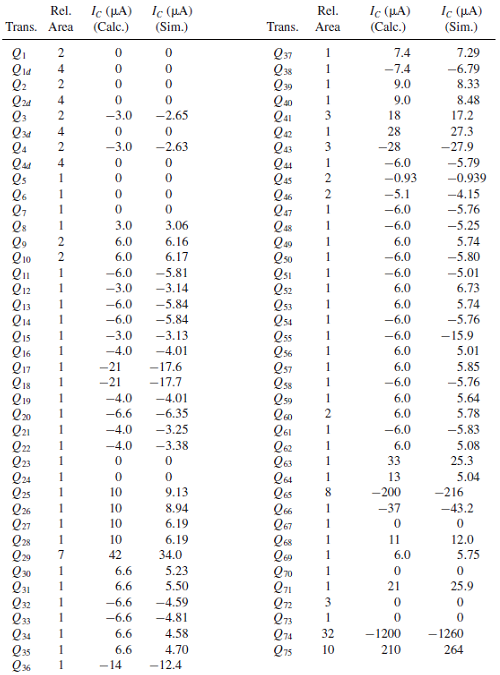
\includegraphics[width=400pt]{./imagenes/642.png}
\end{center}
\caption{Corrientes calculadas y simuladas.}
\label{642}
\end{figure}

Por supuesto que las estimaciones hechas en un principio para las corrientes $I_{C55}$ e $I_{C64}$ podían haberse sustituido por cálculos que contemplaran ya en ese momento a las corrientes de base, sin embargo este procedimiento podría acarrear un significativo nivel de complejidad. En la practica un análisis de primera aproximación permite asumir cierto grado de simplificación. Por ejemplo las corrientes de base siempre pueden despreciarse en los estudios de polarización. Así, después el dispositivo puede ser simulado y mediante la comparación de los resultados con la simulación ello puede indicar el ajuste de algún parámetro que originalmente haya sido despreciado, justo como se ha llevado a cabo en este trabajo. Este procedimiento tiene la ventaja de su simplicidad. Estos análisis simplificados constituyen un método de trabajo muy apropiado en la practica por cuanto el diseño es el procedimiento inverso al análisis. Las hipótesis simplificativas permiten a los diseñadores ajustar sus proyectos realizando rápidas verificaciones de sus comportamientos bajo diferentes condiciones. Estos procedimientos le permiten al diseñador poner énfasis en cada uno de los parámetros que limitan el comportamiento satisfactorio de su proyecto en cada una de dichas condiciones.

\subsection{Transistores que se encuentran normalmente inactivos}

Considere el circuito de la figura \ref{636} y en el que la tensión de entrada de modo común es tal que los transistores $Q_{1}$, $Q_{2}$ y $Q_{6}$ operen la región activa y lineal. Si la tensión  de entrada al amplificador diferencial se incrementa, la corriente de $Q_{2}$ aumenta y la del transistor $Q_{1}$ disminuye. Por lo tanto la tensión entre el nodo 2 y tierra cae y la correspondiente al nodo 1 con referencia de tierra sube. La cuestión es que cuando $Q_{1}$ y $Q_{2}$ operan en la región lineal ellos introducen un desplazamiento de fase de 180 o entre las tensiones de sus colectores y las de sus bases. Ahora suponga que la tensión de entrada de modo común se incrementa hasta alcanzar 100 o 200 mV por debajo de VCC de modo que $Q_{1}$ y $Q_{2}$ pasan a saturación.\\

Bajo estas condiciones la unión colector-base de estos transistores pasan a polarizarse en forma directa, y la tensión presente en dicha juntura permanece aproximadamente constante. En consecuencia, incrementando la tensión de entrada diferencial del Op. Amp. ello produce un incremento en la tensión presente entre el nodo 2 y tierra y simultáneamente una disminución en la tensión del nodo 1 con igual referencia. En otras palabras, la operación de los transistores en saturación hace que los mismos dejen de invertir la fase de las tensiones que normalmente introducían. Invirtiéndose la polaridad de la ganancia de la etapa de entrada se invierte la polaridad de la ganancia del operacional, transformándose una realimentación negativa en positiva con la consiguiente posibilidad de inestabilidad. Un problema similar ocurre cuando la tensión de entrada de modo común alcanza valores tan negativos como -VEE en los que los transistores $Q_{3}$ y $Q_{4}$ pasan a saturación (efecto LATCH UP).\\

Este problema ocurre cuando la tensión de entrada de modo común va mas allá de los limites o rango permitido por el Op. Amp. En principio este problema puede ser subsanado especificando la tensión de entrada de modo común máxima de modo que ningún transistor de entrada pueda llegar a saturar. Sin embargo tomando la precaución de que nunca la polaridad de los terminales de entrada del circuito puedan invertirse se amplia considerablemente el campo de aplicación del Op.Amp.\\

La figura \ref{643} presenta el diagrama esquemático de una parte de la etapa de entrada del NE5234 con los transistores $Q_{1d}$, $Q_{2d}$, $Q_{3d}$ y $Q_{4d}$ los cuales fueran omitidos en la figura \ref{636} por simplicidad. Las uniones base-emisor de estos transistores se encuentran cortocircuitadas, por lo tanto cada uno de estos transistores es en realidad un diodo entre sus terminales de colector y base. Cuando $Q_{1}$ y $Q_{2}$ saturan, sus junturas colector-base se polarizan en directo. La base de $Q_{1d}$ esta conectada a la base de $Q_{1}$ y la base de $Q_{2d}$ se encuentra conectada a la base de $Q_{2}$. Los colectores de $Q_{1d}$ y $Q_{2d}$ se hallan conectados a los colectores de $Q_{1}$ y $Q_{2}$ respectivamente. En consecuencia, con un apareamiento de transistores perfecto y para una tensión de entrada de modo común exclusivamente,  $V_{BC1} = V_{BC1d} = V_{BC2} = V_{BC2d}$ y las uniones colector-base de estos cuatro transistores se encuentran igualmente polarizadas.

\begin{figure}[!h]
\begin{center}
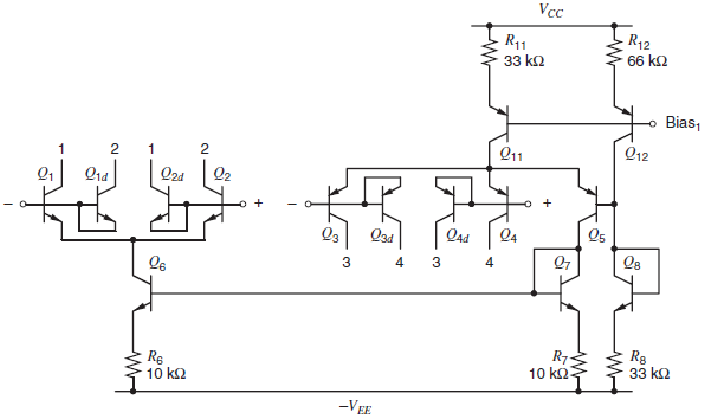
\includegraphics[width=300pt]{./imagenes/neinputdiodos.png}
\end{center}
\caption{Esquema parcial de la etapa de entrada con diodos en ambos pares diferenciales.}
\label{643}
\end{figure}

Para impedir el cambio de polaridad de terminales precedentemente descripto, los transistores $Q_{1d}$ y $Q_{2d}$ poseen mayores áreas semiconductoras que $Q_{1}$ y $Q_{2}$ (en el NE5234 la relación de áreas es 2). Cuando la uniones base-colector comienzan a tener polarización directa, las uniones de $Q_{1d}$ y $Q_{2d}$ conducen una mayor corriente que aquellas de $Q_{1}$ y $Q_{2}$. De este modo, los cambios en la tensión de entrada aplicada al terminal no inversor ejercen mayor influencia en el nodo 1 que en el nodo 2 y los cambios en la tensión de entrada aplicada al terminal inversor producen mayor influencia en el nodo 2 que en el nodo 1. Como consecuencia, cuando la tensión de entrada diferencial se incrementa, la tensión entre el nodo 1 y tierra aumenta mientras que la del nodo 2 disminuye como ocurre en operación normal. Similar comportamiento tiene lugar en el par diferencial pnp. Este circuito permite que el rango de tensión de entrada de modo común pueda extenderse hasta unos 700 mV por debajo de VCC hasta cerca de unos 700 mV por arriba de –VEE. En los extremos alto y bajo unos cientos de mV por debajo de dichos limites, los transistores de la etapa de entrada operan en saturación y en algunos Op.Amp. sus especificaciones no lo aclaran. Sin embargo la ganancia del amplificador operacional no se invierte en fase en el rango precedentemente detallado. Excediéndose dicho rango pueden sobrevenir daños en los transistores $Q_{1d}$, $Q_{2d}$, $Q_{3}$ y $Q_{4}$. Es posible incorporar resistores en serie con estos terminales de entrada para evitar dichos daños limitando la corriente a través de dichos diodos cuando pasan a conducción.\\

Los transistores $Q_{23}$ y $Q_{24}$ en la figura \ref{637} normalmente permanecen cortados. Sus bases se encuentran conectadas al nodo $Bias2$ el cual es una salida del circuito de polarización de la figura \ref{640}. La tensión entre el nodo $Bias2$ y masa es $V_{EB38} = 0,7 V$ aproximadamente. Por lo tanto si las tensiones entre el nodo 9 o el nodo 10 contra masa se incrementara hasta alcanzar 1,4 V cuando una señal diferencial grande es aplicada a los terminales de entrada del amplificador operacional, $Q_{23}$ y $Q_{24}$ pasan a conducción para prevenir posibles ulteriores incrementos en estas tensiones. Esta limitación es muy importante para evitar que los transistores $Q_{16}$ y $Q_{19}$ saturen, reduciendo la demora requerida para un manejo apropiado en caso de una súbita reducción en la magnitud de la tensión diferencial de entrada.\\

Los transistores $Q_{67}$ y $Q_{70}$ en la figura \ref{639} también se encuentran normalmente cortados. Estos transistores pasan a conducción para limitar la corriente a la carga $I_{L}$ y prevenir así la  destrucción de los transistores $Q_{74}$ y $Q_{75}$. Por ejemplo si el transistor $Q_{67}$ se encuentra cortado su tensión base-emisor es

$$ V_{BE67} = |I_{C66}|*R_{67} - I_{C63}*R_{63}$$

El transistor $Q_{67}$ pasa a conducción cuando su tensión base-emisor alcanza $V_{BEu} = 0,7 V$ por lo que rescribiendo la anterior ecuación para esta condición:

$$|I_{C66}| = \frac{V_{BE(on)}}{R_{67}} + I_{C63} * \frac{R_{63}}{R_{67}} = \frac{0,7 V}{1,5 k\Omega} + 33 \mu A * \frac{1,2 k\Omega}{1,5 k\Omega} = 490 \mu A$$

Dado que el área semiconductora del transistor $Q_{74}$ es 32 veces mas grande que la del $Q_{66}$, $Q_{67}$ entrara en conducción cuando

$$|I_{C74}| = 32(490 \mu A) = 12 mA$$

Una vez que $Q_{66}$ entra en conducción , el eleva la caída de tensión en $R_{63}$ disminuyendo así la corriente $I_{C63}$. Este cambio reduce la capacidad del transistor $Q_{63}$ de hacer bajar la tensión de la base de $Q_{65}$, el cual limita la capacidad de $Q_{65}$ para hacer bajar la tensión de la base de $Q_{74}$. Como consecuencia la corriente de este ultimo queda limitada al valor precedentemente estimado de alrededor de $16 \mu A$.\\

Similar comportamiento posee el circuito de limitación de la corriente del transistor $Q_{75}$. La corriente es sensada por $Q_{71}$. Cuando  $I_{C75}$ se hace grande, $Q_{70}$ pasa a conducción tirando hacia abajo la tensión del emisor de $Q_{18}$ en la figura \ref{637}, reduciendo la corriente $I_{C18}$ limitando la corriente que el puede proveer para elevar el potencial del nodo 26 y limitar la corriente $I_{C75}$.\\

Los transistores $Q_{72}$ y $Q_{73}$ en la figura \ref{639} se encuentran normalmente cortados. Su propósito es limitar el grado en que $Q_{74}$ y $Q_{75}$ puedan saturar. Esta limitación es importante ya que permite que los transistores de salida alcancen dicha condición sin acumular excesiva carga de portadores minoritarios en su región de base en modo de no incrementar el tiempo necesario para que pasen a la condición contraria disminuyendo así la distorsión de cruce. Si $Q_{74}$ comienza a saturar su juntura base colector empieza a recibir polarización directa. Como resultado de ello la tensión entre el nodo 25 y masa cambia hacia abajo en 0,7 V por efecto de $Q_{74}$ y simultáneamente para arriba en igual cantidad por $Q_{65}$, $V_{EB72} = 0$ aproximadamente. El transistor $Q_{72}$ pasa a operar en su región activa inversa cuando $Q_{74}$ comienza a saturar. En este modo de operación, la corriente de $Q_{72}$ circula hacia su terminal de colector y sale por su terminal de emisor y hacia el nodo 25. Esta corriente eleva la tensión presente entre este nodo y tierra el cual reduce la tensión de salida y evita aquel efecto cuando $Q_{74}$ satura. Similarmente, cuando el transistor $Q_{75}$ comienza a saturar, su juntura base-colector comienza a polarizarse en forma directa, lo cual polariza en forma directa la juntura base-colector del transistor $Q_{73}$. Este transistor entonces opera en su región activa inversa colectando corriente desde el terminal 26 para reducir la tensión entre dicho nodo y masa y en el limite evitar las consecuencias de la saturación de $Q_{75}$. 

\section{Análisis dinámico de bajo nivel del Op.Amp. NE5234}

Nuestro próximo objetivo es la determinación de las propiedades dinámicas  de bajo nivel del amplificador operacional. Con tal objetivo subdividiremos el circuito en tres partes, la etapa de entrada, la segunda etapa y la etapa amplificadora de salida estudiando cada una de ellas. En esta sección consideraremos $hfe_{npn} = \beta_{npn} = 40$, $hfe_{pnp} = \beta_{pnp} = 10$ y $VA_{npn} = 30 V$ y  $VA_{pnp} = 20 V$ salvo aclaración en contrario. Estos valores son tan solo estimados como limites mínimos de lo que se presenta normalmente en la practica.

\subsection{Etapa de Entrada}

La etapa de entrada de este amplificador diferencial es un circuito totalmente diferencial, formado por dos pares de emisores comunes y su resistencia de entrada depende de cual de los pares están conduciendo. Supongamos que $V_{IC} <  0,8 V$. Entonces el par npn $Q_{1}-Q_{2}$ se encuentra cortado, y $Q_{11}$ se encuentra polarizando al par pnp $Q_{3}-Q_{4}$. La figura \ref{644}. presenta el medio circuito equivalente para este modo de operación. La resistencia de carga es $\frac{R_{in2}}{2}$, la cual es la mitad de la resistencia de entrada de la segunda etapa. Mientras el transistor $Q_{3}$ opera con su emisor a masa de pequeña señal, la resistencia de entrada de este medio circuito diferencial es $h_{ie3}$ y por lo tanto la resistencia de entrada diferencial es:

$$R_{id} = 2 hie_{3}$$

Entonces, dado que $|I_{C11}| = 6 \mu A$, $|I_{C3}| = |I_{C4}| = 3 \mu A$

$$R_{id} = 2 \frac{\beta_{pnp}}{gm_{3}} = 2 \frac{\beta_{pnp}}{|I_{C3}|}V_{T} = 2 \frac{10}{3 \mu A}25 mV = 170 k\Omega$$
	
Para una tensión de entrada diferencial, los terminales de base de $Q_{9}$ y $Q_{13}$ de pequeña señal también están conectados a masa como se puede observar en la figura \ref{644}. Por consecuencia ambos transistores operan como amplificadores base común y como ambos poseen resistencias conectadas en sus terminales de emisor a tierra, sus resistencias de salida que llamaremos $R_{up1}$ para $Q_{13}$ y $R_{down1}$ para $Q_{9}$ resultan:	
	
\begin{figure}[!h]
\begin{center}
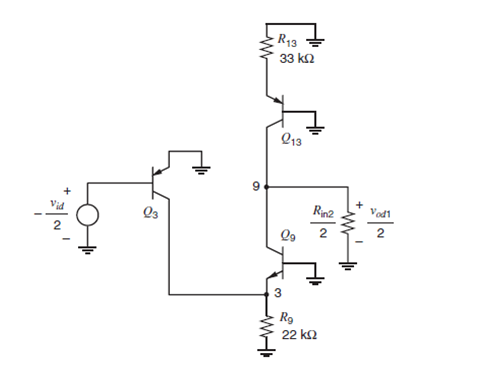
\includegraphics[width=300pt]{./imagenes/diffmode.png}
\end{center}
\caption{Circuito en modo diferencial, etapa de entrada con $V_{IC} << 0,8 V$}
\label{644}
\end{figure}
	
$$R_{up1} = r_{oe13} (1 + hfe_{13} \frac{R_{13}}{R_{13} + R_{B13} + hie_{13}})$$ con $R_{B13} = 0$, así

$$R_{up1} = 3,33*10^{6} (1 + 10 * \frac{33}{3+0+41,6}) = 3,33*10^{6}*5,42 = 18 M\Omega$$

Similarmente, si la resistencia de salida por colector de $Q_{3}$ es mucho mas grande que $R_{9}$, entonces la resistencia de salida $R_{down1}$ es:

$$R_{down1} = r_{oe9} (1 + hfe_{9} \frac{R_{9}}{R_{9} + R_{B9} + hie_{9}})$$ con $R_{B9} = 0$, así

$$R_{down1} = 5*10^{6} (1 + 40 * \frac{22}{22+0+166,4}) = 5*10^{6}*5.42 = 27 M\Omega$$

con la cual, la resistencia de salida de la primer etapa es:

$$Ro_{1} = \frac{R_{up1}}{R_{dowm1}} = \frac{18 M\Omega}{27 M\Omega} = 11 M\Omega$$

La transconductancia diferencial de la primera etapa, que definiremos como  $Gmd1 = \frac{I_{cd9}}{V_{id}}$, dada su carga activa resultara:

$$Gmd1 = gm_{3} \frac{R_{9}}{hib_{9}+R_{9}} = gm_{3} \frac{gm_{9}R_{9}}{1 + gm_{9}R_{9}} = 40*3*10^{-6}*\frac{40*6*10^{-6}*22*10^{3}}{1+40*6*10^{-6}*22*10^{3}} $$

$$Gmd1 = 10 \mu A/V * 0,84 = 100 \mu A/V$$

Como se apunto oportunamente, la transconductancia diferencial de la primera etapa del Op.Amp. no depende de la tensión de entrada de modo común. 

\subsection{Segunda Etapa}

Mientras los potenciales de los nodos 9 y 10 son iguales y de signo contrario cuando la excitación es exclusivamente diferencial,  los emisores de los transistores $Q_{25}$ y $Q_{28}$ se encuentran conectados a tierra para pequeña señal (tierra virtual). Entonces la resistencia de entrada de la segunda etapa resulta ser:

$$R_{i2} = 2 (hie_{21}+(hfe_{21}+1)*\frac{hi2_{25}}{hie_{26}})$$

suponiendo que la resistencia que se observa en el colector de $Q_{16}$ es mucho mayor que $(hie_{25} // hie_{26})$. Dado que $hie_{25} = hie_{26}$

$$R_{i2} = 2*( \frac{10}{40*4*10^{-6}}+\frac{11}{2}*\frac{401}{40*4*10^{-6}} = 1,3 M\Omega$$

Para hallar la resistencia de salida previamente determinaremos la resistencia vista desde los colectores de $Q_{17}$ y $Q_{18}$ hacia arriba del circuito, que llamaremos $R_{up2}$ para luego hacer lo propio con la parte inferior del circuito desde dichos colectores a la que llamaremos $R_{down2}$. En el primer caso se trata de sendos circuitos del tipo $R_{e}$ sin puentear por lo que

$$R_{up2} = r_{oe17} (1 + hfe_{17} \frac{R_{17}}{R_{17} + R_{B17} + hie_{17}})$$ con $R_{B17} = 0$, así

$$R_{up2} = 0,952*10^{6} (1 + 10 * \frac{9,3}{9,3+0+11,9}) = 0,952*10^{6}*5,38 = 5,1 M\Omega$$

Ahora mirando hacia abajo desde los colectores de $Q_{25}$ y $Q_{26}$

$$R_{down2}  = r_{o25} (1 + gm_{25} R_{E25})$$
	
Donde $R_{E25}$ es la resistencia equivalente de pequeña señal que presenta el circuito conectado en el emisor de $Q_{25}$. Suponiendo que la resistencia vista desde el colector de $Q_{29}$ es muy alta como para ser despreciada, $R_{E25}$ es la resistencia vista desde los emisores de $Q_{26}$ y $Q_{28}$. Mientras los colectores de $Q_{27}$ y $Q_{28}$ están conectados a masa para pequeña señal (VCC), la resistencia vista entre cada uno de sus emisores y masa es $hib_{27}$ y $hib_{28} = (1/gm28)$. Sin embargo para $Q_{26}$ su determinación resulta mucho mas complicada por cuanto la resistencia conectada en su colector puede ser muy grande. Llamemos $R_{in3}$ a la resistencia de entrada de la tercer etapa en el nodo 26, entonces $R_{E25}$ es	

$$R_{E25} = (r_{e26} + \frac{\beta_{0npn}}{\beta_{0npn} + 1} * \frac{R_{up2}||R_{in3(26)}}{gm_{26}*r_{026}})||r_{e27}||r_{e28}$$

con $r_{e} = h_{ib} = \frac{1}{gm}$

Si $(R_{in3(26)} / gm_{26}*r_{o26}) << r_{e26}$  que se convierte en realidad debido al bajo valor de $\beta_{0npn}$ aquí supuesto entonces:

$$R_{E25} \approx \frac{\beta_{0npn}}{\beta_{0npn} + 1} * (\frac{1}{gm_{26}}||\frac{1}{gm_{27}}||\frac{1}{gm_{28}})$$

$$R_{E25} \approx \frac{40}{41}* (\frac{26mV}{10 \mu A}||\frac{26mV}{10 \mu A}||\frac{26mV}{10 \mu A}) = 0,85 k\Omega$$

Sustituyendo este resultado en la ecuación anterior de $R_{down2}$:

$$R_{down2} = \frac{30 V}{10 \mu A} * (1 + \frac{10 \mu A}{26 mV} 0,85 k\Omega) = 4 M\Omega$$

Como resultado de ello la resistencia de salida de la segunda etapa vista hacia adentro del terminal 25 resulta:

$$R_{o2} = R_{up2}||R_{down2} = 2.2 M\Omega$$

La figura \ref{645} representa el circuito equivalente de la segunda etapa preparado para la determinación de la transconductancia de la misma. El resistor identificado como $R_{up2}$ representa la resistencia de pequeña señal vista desde el colector de $Q_{17}$ o de $Q_{18}$ en el circuito de la figura \ref{637}. Dicha resistencia fue calculada precedentemente y su resultado fue de $5 M\Omega$ cada una. Las resistencias rotuladas como $R_{in3(25)}$ y $R_{in3(26)}$ como se dijo precedentemente representan las resistencias de entrada de la tercera etapa en los terminales 25 y 26, respectivamente. Llamemos $V_{9}$, $V_{10}$ y $V_{25}$  a las diferencias de potencial de pequeña señal referidas a masa en los nodos 9, 10 y 25, respectivamente. Los emisores de los transistores $Q_{25} - Q_{28}$ se encuentran flotantes en la figura \ref{645} por cuanto $Q_{29}$ en la figura \ref{637} opera como una fuente de corriente con una resistencia de salida mucho mas grande que la resistencia vista hacia dentro de los emisores de $Q_{25} - Q_{28}$.  Llamemos $av21$ y $av22$ a las ganancia de tensión de pequeña señal de los seguidores por emisor $Q_{21}$ y $Q_{22}$ en la figura \ref{637}, respectivamente.

\begin{figure}[!h]
\begin{center}
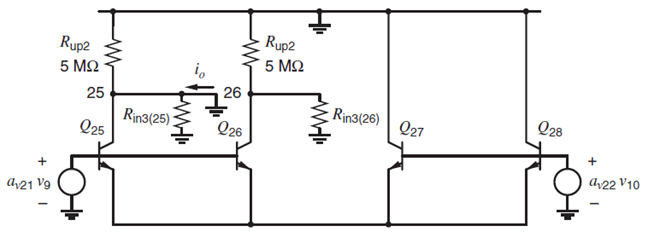
\includegraphics[width=300pt]{./imagenes/ssofsecsta.png}
\end{center}
\caption{Modelo de pequeña señal, segunda etapa para hallar su transconductancia.}
\label{645}
\end{figure}

Cada seguidor de emisor tiene como carga $R_{L} = hie_{25}//hie_{26} = hie_{27}//hie_{28} = hie_{25}/2$ por lo que las mencionadas ganancias de tensión de dichas etapas resultan:

$$av21 = av22 = \frac{(hfe_{21} + 1) * (roe_{21}||(hie_{25}/2)))}{hie_{21} + ((hfe_{21} + 1) * (roe_{21}||(hie_{25}/2)))}$$

$$av21 = av22 = \frac{11 * (\frac{40*26mV}{2*10 \mu A}||\frac{20V}{4 \mu A})}{\frac{10*26 mV}{4 \mu A} + 11 * (\frac{40*26mV}{2*10 \mu A}||\frac{20V}{4 \mu A})}$$

$$av21 = av22 = 0,90$$

La transconductancia de la segunda etapa la definimos como (con $v_{25} = 0$):

$$G_{m2} = \frac{i_{0}}{v_{9} - v_{10}}$$

Por cuanto la tensión de modo común de salida de la primera etapa se fija en un valor constante, tal como se mostró en la figura \ref{638},  $v_{9} = vod1-2$ y $v_{10} = - vod1-2$, donde $vod1$ es la tensión de modo diferencial de salida de la primera etapa. Por simplicidad en la búsqueda de la transconductancia de esta segunda etapa, asumiremos que $v_{10} = 0$. Este cambio introduce una tensión de modo común no nula en la entrada de la segunda etapa. Sin embargo esta entrada de modo común causa un muy pequeño cambio en $G_{m2}$ debido a que la fuente de corriente $Q_{29}$ de polarización de la segunda etapa posee una muy elevada resistencia de salida. Imponiendo $v_{10} = 0$ también reduce la tensión de entrada diferencial a la segunda etapa a la mitad pero como el modelo de pequeña señal es lineal ello se vera compensado al considerar también la mitad de la corriente de salida $i_{o}$  y no cambia el valor de $G_{m2}$. Como resultado

$$G_{m2} = \frac{i_{0}}{v_{9}}$$

Debido a la característica de linealidad del circuito equivalente de pequeña señal para la determinación de la corriente $i_{o}$ es posible aplicar el teorema de superposición. La figura \ref{646} presenta un circuito equivalente adecuado para la determinación de la primera de las componentes de $i_{o}$.

\begin{figure}[!h]
\begin{center}
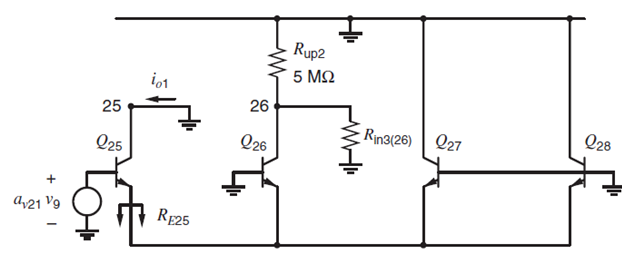
\includegraphics[width=300pt]{./imagenes/646.png}
\end{center}
\caption{Modelo de pequeña señal para hallar la primer componente de $i_{o}$.}
\label{646}
\end{figure}

Los terminales de base de los transistores $Q_{25}$ y $Q_{26}$ son excitados separadamente, y la base de $Q_{26}$ se halla conectada a masa  de pequeña señal en este paso en que se intenta determinar la primera de las componentes $i_{o1}$0. Las resistencias conectadas al nodo 25 se han eliminado ya que la corriente $i_{o1}$ circula por ellas. Para hallar $i_{o1}$ el transistor $Q_{25}$ responde a la configuración tipo emisor común con resistencia de emisor sin puentear. La resistencia equivalente dinámica total conectada en el terminal de emisor de $Q_{25}$ en los cálculos previos la hemos llamado $R_{E25} = 0,85 k\Omega$. A partir de las características de transferencia de dicha configuración amplificadora:

$$i_{o1} = \frac{gm_{25}}{1 + gm_{25}R_{E25}} * av21*v_{9}$$

La figura \ref{647} presenta el circuito equivalente adecuado para la determinación de la segunda de las componentes de la corriente $i_{o}$ en este segundo paso.

\begin{figure}[!h]
\begin{center}
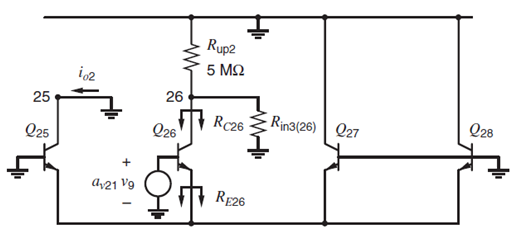
\includegraphics[width=300pt]{./imagenes/647.png}
\end{center}
\caption{Modelo de pequeña señal para hallar la segunda componente de $i_{o}$.}
\label{647}
\end{figure}

Aquí el terminal de base del transistor $Q_{25}$ se encuentra conectado a masa de señal. Para determinar la corriente de colector del transistor $Q_{26}$ que llamamos $ic_{26}$ este transistor $Q_{26}$ se presenta como una nueva configuración amplificadora tipo emisor común con resistencia de emisor sin puentear. La resistencia total y equivalente conectada en el nodo de emisor del transistor $Q_{26}$ que llamamos $R_{E26}$ corresponde al paralelo de la resistencia de entrada de tres transistores $Q_{27}$,$Q_{28}$ y $Q_{25}$ en configuración base común por lo que.

$$R_{E26} = h_{ib27} || h_{ib28} || h_{ib25} = \frac{h_{ib27}}{3} = 0,85 k\Omega$$

Entonces la resistencia de salida por colector de $Q_{26}$ dada dicha resistencia de emisor resulta ser:

$$R_{C26} = r_{o26} (1 + gm_{26} R_{E26}) = \frac{30 V}{10 \mu A} * (1 + \frac{10 \mu A}{26 mV}*0,85 k\Omega) = 4 M\Omega$$

Para hallar la corriente de colector de $Q_{26}$ hay que considerar el divisor resistivo de corriente que se observa conectado en el nodo de colector de dicho transistor, de modo que:

$$i_{c26} \approx \frac{gm_{26}}{1 + gm_{26}R_{E26}} * av21*v_{9} * \frac{R_{C26}}{R_{C26} + R_{up2}||R_{in3(26)}}$$

$$i_{c26} \approx \frac{gm_{26}}{1 + gm_{26}R_{E26}} * av21*v_{9}$$

en donde se ha considerado que $R_{in3(26)} << R_{C26}$ en la ultima aproximación.\\

Debido a que los transistores $Q_{27}$,$Q_{28}$ y $Q_{25}$ son tres transistores idénticos con sus terminales de base conectados a masa, la corriente $ic_{26}$ se divide en tres partes iguales de modo que la parte $i_{o2}$ resulta ser

$$G_{m2} \approx av21 * (\frac{gm_{25}}{1 + gm_{25}R_{E25}} - \frac{gm_{26}}{3*(1 + gm_{26}R_{E26})}$$

$$G_{m2} \approx 0.9 * (\frac{\frac{10 \mu A}{26 mV}}{1 + \frac{10 \mu A}{26 mV}*0,85 k\Omega} - \frac{\frac{10 \mu A}{26 mV}}{3*(1 + \frac{10 \mu A}{26 mV}*0,85 k\Omega)})$$

$$G_{m2} \approx 170 \frac{\mu A}{V}$$

La transconductancia así calculada se obtuvo tomando al nodo 25 como terminal de salida de la segunda etapa. Para el circuito que considere como salida al nodo 26 esta misma transconductancia es aplicable tanto como $R_{in3(26)} = R_{in3(25)}$. Cuando $I_{C74} >> I_{C75}$ o $I_{C74} << I_{C75}$ la polarización con realimentación o estabilización en la etapa de salida duplica esta transconductancia para la vía de excitación de salida como se describió antes.


\subsection{Etapa de salida}

En la sección 1.1 hemos adoptado como corriente de carga $I_{L} = 1 \mu A$. En este caso el circuito de polarización de la etapa de salida regula la corriente de colector del transistor $Q_{75}$ para que sea siempre constante. Mientras $Q_{75}$ es excitado por el seguidor de emisor $Q_{68}$, la corriente de base de $Q_{68}$ debe permanecer constante bajo estas condiciones. Para describir este resultado consideraremos el circuito de la figura \ref{648} el cual presenta el circuito equivalente de pequeña señal de la parte principal de la segunda etapa mas la etapa diferencial $Q_{39}$ - $Q_{40}$ proveniente del circuito de polarización que controla a la etapa de salida.

\begin{figure}[!h]
\begin{center}
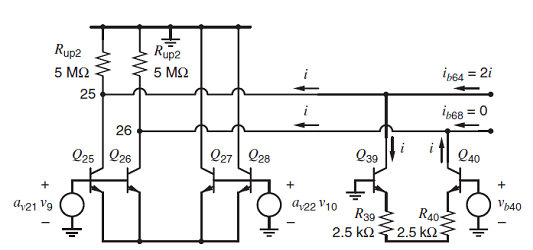
\includegraphics[width=300pt]{./imagenes/648.png}
\end{center}
\caption{Modelo de pequeña señal para hallar la segunda componente de $i_{o}$.}
\label{648}
\end{figure}

La salida de este modelo circuital son los terminales 25 y 26 que excitan las bases de los transistores $Q_{64}$ y $Q_{68}$ en la figura \ref{639}.\\ 

Primero consideremos la segunda etapa. Los terminales de salida son excitados por un circuito totalmente balanceado, y la carga conectada en los mismos en la tercer etapa también lo es. Por lo tanto la corriente de pequeña señal que fluye hacia los nodos 25 y 26, rotulada como corriente $i$ en la figura \ref{648} tiene igual valor en ambos terminales.\\

Ahora consideremos el par diferencial $Q_{39}$ – $Q_{40}$. Este par conforma una etapa de entrada de un amplificador diferencial que opera dentro de un lazo de realimentación negativa que mantiene $I_{C75}$ siempre constante cuando $I_{C74} >> I_{C75}$, tal como se ha descripto con anterioridad. En la figura \ref{648} la base del transistor $Q_{39}$ esta referida a masa de señal  por cuando las corrientes de colector de los transistores $Q_{37}$ y $Q_{38}$ en la figura \ref{640} son constantes. Por otro lado la base del transistor $Q_{40}$ es excitada por una diferencia de potencial de señal rotulada como $vb40$ aplicada entre dicha base y masa. Mientras $Q_{75}$ es excitada por $Q_{68}$ manteniendo constante a la corriente $I_{C75}$, lo cual significa que la componente de corriente de señal  en la base de $Q_{68}$, es decir $i_{b68}$ debe ser nula aproximadamente. Por lo tanto $Q_{40}$ debe inyectar una corriente de señal $i$ hacia el nodo 26 bajo estas condiciones tal como muestra la figura \ref{648}. En razón de que la corriente total del par diferencial es constante, $Q_{39}$ debe inyectar la misma corriente i al nodo 25. Este resultado duplica el valor de la corriente de pequeña señal en la base de $Q_{64}$, $i_{b64}$, llevándolo a (2.i) ,  doblando efectivamente el valor de $G_{m2}$ para la salida 25 y haciendo cero a la transconductancia $G_{m2}$ en la salida 26 cuando $I_{C74} >> I_{C75}$. Por lo tanto en el estudio del comportamiento de la etapa de salida se pondrá énfasis en  la parte circuital que tiene como entrada al nodo 25 . En el caso opuesto (es decir $I_{C74} << I_{C75}$) la parte que tiene al terminal 26 como entrada es la parte predominante. Cuando $I_{C74} = I_{C75}$ ambos trayectos deben ser considerados.\\

Ignorando la resistencia vista hacia abajo del colector de \ref{639},  la resistencia de entrada de la tercer etapa (\ref{639}) en el nodo 25 es:

$$R_{i3(25)} = hie_{64} + (hfe_{64} + 1)*R_{E64}$$

En esta ecuación $R_{E64}$ es la resistencia dinámica presente en el emisor de $Q_{64}$, la cual es:

$$R_{E64} = r_{o63}*(1+gm_{63}R_{63}))||(r_{\pi 65}+(\beta_{0pnp}+1)*R_{E65})$$

Similarmente, $R_{E65}$ es la resistencia dinámica conectada en el terminal de emisor contra masa. Ignorando la resistencia vista desde la base del transistor $Q{43}$ en la figura \ref{640}, $R_{E65}$ es

$$R_{E65} = R_{65} || hie_{66} || hie_{74} = R_{65} || \frac{hfe_{66} V_{T}}{I_{C66}} || \frac{hfe_{74} V_{T}}{I_{C74}}$$

Dado que el área de emisor del transistor $Q_{74}$ es treinta y dos (32) veces mas grande que la del transistor $Q_{66}$:

$$|I_{C66}| = \frac{|I_{C74}|}{32} = \frac{1200 \mu A}{32} = 37 \mu A$$

con lo cual:

$$R_{E65} = 7,5 k\Omega || \frac{10*26 mV}{37 \mu A} || \frac{10*26 mV}{1200 \mu A} = 200 \Omega$$

entonces:

$$R_{E64} = \left \{ \frac{30 V}{33 \mu A} * (1 + \frac{33 \mu A}{26 mV} * 1,2 k\Omega)\right \} || \left \{ \frac{10*26 mV}{200 \mu A} + 11*200 \Omega)\right \} = 3,5 k\Omega$$

con lo cual reemplazando en la ecuación de $R_{i3(25)}$ y teniendo en cuenta además que tal como se calculo previamente $I_{C64} = 4 \mu A$.

$$R_{i3(25)} = \frac{40*26 mV}{4 \mu A} + 41*3,5 k\Omega = 404 k\Omega$$

La resistencia de salida de este etapa

$$R_{o3} = r_{o74} || r_{o75} = \frac{40 V}{1200 \mu A} || \frac{30 V}{210 \mu A} = 15 k\Omega$$

La transconductancia de esta etapa es:

$$G_{m3} = a_{v64}*a_{v65}*g_{m74}$$

Donde $a_{v64}$ y $a_{v65}$ son las ganancias de tensión de los seguidores de emisor $Q_{64}$ y $Q_{65}$, respectivamente. Dado que $r_{o64} >> R_{E64}$:

$$a_{v64} = \frac{(hfe_{64} + 1)*R_{E64}}{hie_{64} + [(hfe_{64} + 1)*R_{E64}]} = \frac{41*3,5*10^{3}}{\frac{40*26 mV}{4 \mu A} + 41*3,5*10^{3}} = 0,36$$

Dado que $r_{o65} >> R_{E65}$:

$$a_{v65} = \frac{(hfe_{65} + 1)*R_{E65}}{hie_{65} + [(hfe_{65} + 1)*R_{E65}]} = \frac{11*200}{\frac{10*26 mV}{200 \mu A} + 11*200} = 0,63$$

En consecuencia:

$$G_{m3} = 0,36 * 0,63 * \frac{100 \mu A}{26 mV} = \frac{1}{96 \Omega}$$

\subsection{Ganancia de lazo abierto del operacional}

La ganancia de tensión de la primera etapa cuando se encuentra cargada por la segunda:

$$a_{v1} = G_{m1} * (R_{o1} || \frac{R_{i2}}{2}) = 97 \frac{\mu A}{V} * (11 M\Omega || \frac{1,3 M\Omega}{2}) = 60$$

La ganancia de tensión de la segunda etapa cuando se encuentra cargado por la tercera:

$$a_{v2} = 2 G_{m2} * (R_{o2} || R_{i3(25)}) = 2 * 170 \frac{\mu A}{V} * (2,2 M\Omega || 404 k\Omega) = 120 $$

En la ecuación anterior la transconductancia $G_{m2}$ se ha multiplicado por dos (2) debido al efecto de la polarización con realimentación (estabilización) antes detallado. La ganancia de tensión de la tercera etapa cuando la misma se encuentre cargada por una resistencia equivalente de carga $R_{L} = 2 k\Omega$ por la que circula una corriente de $1 \mu A$ es:

$$a_{v3} = G_{m3}(R_{o3}||R_{L}) = \frac{1}{96 \Omega}*(15 k\Omega || 2 k\Omega) = 18$$

Finalmente, la ganancia a lazo abierto del amplificador operacional tipo NE5234 resulta ser:

$$a_{v} = a_{v1}*a_{v2}*a_{v3} = 130000$$

Esta ganancia es en realidad el mínimo valor de ganancia que pueda presentarse en estos circuitos integrados en razón de que se ha tomado el mínimo valor de resistencia de carga $R_{L}$ bajo el cual se aseguran todas las especificaciones del mismo, y además en estos cálculos se han empleado los mínimos valores de tensiones de Early y ganancias de corriente de todos los transistores que puedan aparecer en esta tecnología y por lo tanto los valores típicos de ganancia son mucho mayores. Igual comentario vale para los resultados obtenidos de $R_{id}$ y $R_{o3}$ que se han recuadrado.

\end{document}